\documentclass[a4paper]{article}

\usepackage{polski}
\usepackage[utf8]{inputenc}
\usepackage[pdftex]{graphicx}
\usepackage{fancyhdr}
\usepackage{float}

\newcommand{\prog}{\texttt}

\linespread{1.15}
\pagestyle{fancy}
\fancyhf{}
\chead{Specyfikacja implementacyjna}
\cfoot{Strona \thepage \ z \pageref{end}}

\title{Specyfikacja implementacyjna \\ Projekt \textit{Aplikacja OnePass} w języku Python}
\author{Jakub Czajka (299239)}

\begin{document}
\maketitle
\thispagestyle{empty}
\tableofcontents

\newpage

\section{Informacje ogólne}
\subsection{Ogólne parametry uruchomieniowe programu}
Język programowania: \textit{Python}.\medskip\\
Środowisko uruchomieniowe: \textit{dowolny system operacyjny obsługujący Pythona}.\medskip\\
Wielkość okna: \textit{800 x 600 px}.\medskip\\
Położenie okna po uruchomieniu: \textit{środek ekranu}.

\subsection{Konwencja pisania kodu}
Kod programu będzie pisany zgodnie z poniższymi zasadami:
\begin{itemize}
    \item Kod pisany jest z poszanowaniem zasad czystego kodu.
    \item Nazwy są nazwami znaczącymi.
    \item Nazwy są pisane w języku angielskim.
    \item Nazwy klas są pisane w konwencji \textit{UpperCamelCase}.
    \item Nazwy metod i zmiennych są pisane małymi literami. Jeżeli składają się z kilku słów, słowa oddzielane są znakami \textit{"\_"}.
\end{itemize}

\section{Opis modułów i danych}
\subsection{Moduły w programie}
Mój program jest podzielony na trzy odrębne moduły:

\subsubsection{Graficzny interfejs użytkownika}
Moduł ten odpowiedzialny jest za interaktywną i graficzną komunikację z użytkownikiem programu. Jego głównym zadaniem jest przedstawianie zawartości aplikacji oraz umożliwienie użytkownikowi komunikację z programem w łatwy sposób. Moduł ten połączony jest z modułem kontrolerów.

\subsubsection{Kontrolery}
Moduł ten odpowiedzialny jest za komunikację aplikacji między modułami. Łączy moduł graficznego interfejsu użytkownika z modułem obilczeń aplikacji.

\subsubsection{Obliczenia}
Moduł ten odpowiedzialny jest za pracę aplikacji. W tym miejscu przetwarzane są dane, wykonuje się szyfrowanie i deszyfrowanie oraz przechowuje się dane. Moduł ten komunikuje się z modułem kontrolerów.

\section{Opis klas}
\subsection{Model}

\subsubsection{MProfile}
\begin{description}
    \item[Pakiet:] model
    \item[Dziedziczy:] --
    \item[Konstruktor:] otrzymuje zmienne typu \prog{string} zawierające dane osobowe. Ustawia je w odpowiednie pola klasy.
    \item[Pola:] \hfill
    \begin{itemize}
        \item \prog{string name} -- przechowuje imię użytkownika.
        \item \prog{string surname} -- przechowuje nazwisko użytkownika.
        \item \prog{string email} -- przechowuje email użytkownika.
        \item \prog{string login} -- przechowuje login użytkownika.
        \item \prog{string hasło} -- przechowuje hasło użytkownika.
        \item \prog{List passwords} -- przechowuje obiekty haseł użytkownika.
        \item \prog{List notes} -- przechowuje notatki użytkownika.
    \end{itemize}
    \item[Metody:] \hfill
    \begin{itemize}
        \item \textbf{Prototyp:} \prog{public void update(string update)}\\\textbf{Zadanie:} zaktualizowanie informacji o użytkowniku.
        \item \textbf{Prototyp:} \prog{public void update\_passwords(List update)}\\\textbf{Zadanie:} zaktualizowanie informacji o hasłach.
        \item \textbf{Prototyp:} \prog{public void update\_notes(List update)}\\\textbf{Zadanie:} zaktualizowanie informacji o notatkach.
    \end{itemize}
\end{description}

\subsubsection{MPassword}
\begin{description}
    \item[Pakiet:] model
    \item[Dziedziczy:] --
    \item[Konstruktor:] otrzymuje zmienne typu \prog{string} zawierające dane hasła. Ustawia je w odpowiednie pola klasy.
    \item[Pola:] \hfill
    \begin{itemize}
        \item \prog{string name} -- przechowuje nazwę hasła.
        \item \prog{string login} -- przechowuje login.
        \item \prog{string password} -- przechowuje hasło.
        \item \prog{string url} -- przechowuje adres do strony.
        \item \prog{boolean is\_favourite} -- przechowuje wartość logiczną opisującą to~czy element jest elementem \textit{ulubionym}.
    \end{itemize}
    \item[Metody:] \hfill
    \begin{itemize}
      \item \textbf{Prototyp:} \prog{public void update(string update)}\\\textbf{Zadanie:} zaktualizowanie informacji o obiekcie.
    \end{itemize}
\end{description}

\subsubsection{MNote}
\begin{description}
    \item[Pakiet:] model
    \item[Dziedziczy:] --
    \item[Konstruktor:] otrzymuje zmienne typu \prog{string} zawierające dane notatki. Ustawia je w odpowiednie pola klasy.
    \item[Pola:] \hfill
    \begin{itemize}
        \item \prog{string name} -- przechowuje nazwę pliku (nazwa notatki plus rozszerzenie).
        \item \prog{string text} -- przechowuje treść notatki.
    \end{itemize}
    \item[Metody:] \hfill
    \begin{itemize}
        \item \textbf{Prototyp:} \prog{public void update(string update)}\\\textbf{Zadanie:} zaktualizowanie danych notatki.
    \end{itemize}
\end{description}

\subsubsection{MHasher}
\begin{description}
    \item[Pakiet:] model
    \item[Dziedziczy:] --
    \item[Konstruktor:] bezargumentowy.
    \item[Pola:] brak
    \item[Metody:] \hfill
    \begin{itemize}
        \item \textbf{Prototyp:} \prog{public string hash(string msg)}\\\textbf{Zadanie:} haszowanie podanej jako argument wiadomość.\\\textbf{Algortym:} SHA256
    \end{itemize}
\end{description}

\subsubsection{MGenerator}
\begin{description}
    \item[Pakiet:] model
    \item[Dziedziczy:] --
    \item[Konstruktor:] bezargumentowy.
    \item[Pola:] brak
    \item[Metody:] \hfill
    \begin{itemize}
        \item \textbf{Prototyp:} \prog{public string generate(tuple parameters)}\\\textbf{Zadanie:} generowanie hasła na podstawie kryteriów przekazanych jako argument w postaci krotki.
    \end{itemize}
\end{description}

\subsubsection{MChecker}
\begin{description}
    \item[Pakiet:] model
    \item[Dziedziczy:] --
    \item[Konstruktor:] bezargumentowy. Inicjuje pola.
    \item[Pola:] \hfill
    \begin{itemize}
        \item \prog{MHasher hasher} -- przechowuje obiekt typu \prog{MHasher}.
    \end{itemize}
    \item[Metody:] \hfill
    \begin{itemize}
        \item \textbf{Prototyp:} \prog{public boolean verify\_data(string data)}\\\textbf{Zadanie:} sprawdzenie poprawność podanego hasła. W tym celu wykorzystuje obiekt typu \prog{MHasher}.
    \end{itemize}
\end{description}

\subsubsection{MProfileMaker}
\begin{description}
    \item[Pakiet:] model
    \item[Dziedziczy:] --
    \item[Konstruktor:] bezargumentowy.
    \item[Pola:] \hfill
    \begin{itemize}
        \item \prog{MHasher hasher} -- przechowuje obiekt służący do zahaszowania hasła podanego przez użytkownika.
    \end{itemize}
    \item[Metody:] \hfill
    \begin{itemize}
        \item \textbf{Prototyp:} \prog{public boolean check\_data(string data)}\\\textbf{Zadanie:} sprawdzenie poprawność podanych danych przy rejestracji.
        \item \textbf{Prototyp:} \prog{private string hash\_password(string password)}\\\textbf{Zadanie:} hashowanie podanego jako argument hasła.
        \item \textbf{Prototyp:} \prog{private MProfile make\_profile()}\\\textbf{Zadanie:} utworzenie nowego obiektu typu \prog{MProfile} z danych podanych przy rejestracji.
    \end{itemize}
\end{description}

\subsubsection{MLoader}
\begin{description}
    \item[Pakiet:] model
    \item[Dziedziczy:] --
    \item[Konstruktor:] bezargumentowy.
    \item[Pola:] \hfill
    \begin{itemize}
        \item \prog{List files} -- przechowuje listę nazw plików zaszyfrowanych.
        \item \prog{List notes} -- przechowuje listę nazw notatek zaszyfrowanych.
    \end{itemize}
    \item[Metody:] \hfill
    \begin{itemize}
        \item \textbf{Prototyp:} \prog{public void load\_logins()}\\\textbf{Zadanie:} załadowanie plik z loginami do programu.
        \item \textbf{Prototyp:} \prog{public MProfile load\_profiles()}\\\textbf{Zadanie:} załadowanie plik z profilem do programu.
    \end{itemize}
\end{description}

\subsubsection{MEncryptor}
\begin{description}
    \item[Pakiet:] model
    \item[Dziedziczy:] --
    \item[Konstruktor:] bezargumentowy.
    \item[Pola:] \hfill
    \begin{itemize}
        \item \prog{List notes} -- przechowuje listę nazw plików z notatkami.
        \item \prog{List passwords} -- przechowuje listę haseł do zaszyfrowania.
        \item \prog{MProfile profile} -- przechowuje obiekt zawierający informacje o~profilu.
    \end{itemize}
    \item[Metody:] \hfill
    \begin{itemize}
        \item \textbf{Prototyp:} \prog{public string decrypt(string file)}\\\textbf{Zadanie:} rozszyfrowanie podanego pliku.\\\textbf{Algorytm:} AES128
        \item \textbf{Prototyp:} \prog{public string encrypt(string file)}\\\textbf{Zadanie:} szyfrowanie podanego łańcucha.\\\textbf{Algorytm:} AES128
    \end{itemize}
\end{description}

\subsection{Presenter}
Pakiet \textit{Presenter} zawiera klasy odpowiadające za sterowanie ekranami i połączenie z pakietem \textit{Model}. Działanie większość metod klas znajdujących się w tym pakiecie sprowadza się do reakcji na naciśnięty przycisk w GUI.\\
Każda klasa ma w sobie pola ekranów które może wyświetlić.
\subsubsection{PMainWin}
\textit{<<klasa abstrakcyjna>>}
\begin{description}
    \item[Pakiet:] presenter
    \item[Dziedziczy:] --
    \item[Konstruktor:] bezargumentowy.
    \item[Pola:]brak
    \item[Metody:] \hfill
    \begin{itemize}
        \item \textbf{Prototyp:} \prog{public void encrypt\_file\_button\_handle()}\\\textbf{Zadanie:} zamiana bieżącej sceny na ekran szyfrowania plików podanych przez użytkownika.
        \item \textbf{Prototyp:} \prog{public void generate\_button\_handle()}\\\textbf{Zadanie:} zamiana bieżącej sceny na ekran generowania hasła.
        \item \textbf{Prototyp:} \prog{public void home\_button\_handle()}\\\textbf{Zadanie:} zamiana bieżącej sceny na ekran główny po zalogowaniu.
        \item \textbf{Prototyp:} \prog{public void note\_button\_handle()}\\\textbf{Zadanie:} zamiana bieżącej sceny na ekran z listą notatek.
        \item \textbf{Prototyp:} \prog{public void password\_button\_handle()}\\\textbf{Zadanie:} zamiana bieżącej sceny na ekran z listą haseł.
    \end{itemize}
\end{description}
Klasa \prog{PMainWin} jest klasą abstrakcyjną, po której dziedziczą następujące klasy:
\begin{itemize}
    \item PMainWinAfter
    \item PPasswordListWin
    \item PNoteListWin
    \item PEncryptWin
\end{itemize}

\subsubsection{PMainWinBefore}
\begin{description}
    \item[Pakiet:] presenter
    \item[Dziedziczy:] --
    \item[Konstruktor:] bezargumentowy. Inicjuje pola.
    \item[Pola:] \hfill
    \begin{itemize}
        \item \prog{MLoader loader} -- przechowuje obiekty załadowujący loginy.
        \item \prog{string logins} -- pole przechowujące załadowane loginy.
    \end{itemize}
    \item[Metody:] \hfill
    \begin{itemize}
        \item Metody odpowiedzialne za reakcje na kliknięcie przycisku:
        \begin{itemize}
            \item about\_app\_button\_handle()
            \item sign\_up\_button\_handle()
            \item sign\_in\_button\_handle()
            \item generate\_button\_handle()
        \end{itemize}
        \item \textbf{Prototyp:} \prog{private string load\_logins()}\\\textbf{Zadanie:} wpisanie w pole \prog{logins} zawartości pliku z loginami.
    \end{itemize}
\end{description}

\subsubsection{PSignInWin}
\begin{description}
    \item[Pakiet:] presenter
    \item[Dziedziczy:] --
    \item[Konstruktor:] bezargumentowy. Inicjuje pola.
    \item[Pola:] \hfill
    \begin{itemize}
        \item \prog{MProfile profile} -- przechowuje obiekt profilu.
        \item \prog{string logins} -- pole przechowujące załadowane loginy.
        \item \prog{MLoader loader} -- pole przechowujące załadowujący profil.
        \item \prog{MChecker checker} -- pole przechowujące obiekt sprawdzający poprawność danych.
    \end{itemize}
    \item[Metody:] \hfill
    \begin{itemize}
        \item Metody odpowiedzialne za reakcje na kliknięcie przycisku:
        \begin{itemize}
            \item forget\_button\_handle()
            \item sign\_up\_button\_handle()
            \item sign\_in\_button\_handle()
        \end{itemize}
        \item \textbf{Prototyp:} \prog{private void validate\_data(string data)}\\\textbf{Zadanie:} wywołanie metody sprawdzającej poprawność danych.
        \item \textbf{Prototyp:} \prog{private void load\_profile(string data)}\\\textbf{Zadanie:} wywołanie metody pobierającej dane, deszyfrującej je i tworzącej obiekt typu \prog{MProfile}.
    \end{itemize}
\end{description}

\subsubsection{PSignUpWin}
\begin{description}
    \item[Pakiet:] presenter
    \item[Dziedziczy:] --
    \item[Konstruktor:] bezargumentowy. Inicjuje pola.
    \item[Pola:] \hfill
    \begin{itemize}
        \item \prog{MProfileMaker profile\_maker} -- przechowuje obiekt tworzący profil.
    \end{itemize}
    \item[Metody:] \hfill
    \begin{itemize}
        \item Metody odpowiedzialne za reakcje na kliknięcie przycisku:
        \begin{itemize}
            \item sign\_up\_button\_handle()
        \end{itemize}
        \item \textbf{Prototyp:} \prog{private void validate\_data(string data)}\\\textbf{Zadanie:} wywołanie metody sprawdzającej poprawność danych.
    \end{itemize}
\end{description}

\subsubsection{PGenerateWin}
\begin{description}
    \item[Pakiet:] presenter
    \item[Dziedziczy:] --
    \item[Konstruktor:] bezargumentowy. Inicjuje pola.
    \item[Pola:] \hfill
    \begin{itemize}
        \item \prog{MGenerator generator} -- przechowuje obiekt generujący hasła.
        \item \prog{VGenerateWin generate\_win} -- przechowuje obiekt okna generacji.
    \end{itemize}
    \item[Metody:] \hfill
    \begin{itemize}
        \item Metody odpowiedzialne za reakcje na kliknięcie przycisku:
        \begin{itemize}
            \item generate\_button\_handle(tuple parameters)
        \end{itemize}
    \end{itemize}
\end{description}

\subsubsection{PPasswordListWin}
\begin{description}
    \item[Pakiet:] presenter
    \item[Dziedziczy:] --
    \item[Konstruktor:] bezargumentowy. Inicjuje pola.
    \item[Pola:] \hfill
    \begin{itemize}
        \item \prog{MProfile profile} -- przechowuje obiekt zwierający informacje o profilu.
    \end{itemize}
    \item[Metody:] \hfill
    \begin{itemize}
        \item Metody odpowiedzialne za reakcje na kliknięcie przycisku:
        \begin{itemize}
            \item add\_button\_handle()
            \item choose\_button\_handle()
        \end{itemize}
    \end{itemize}
\end{description}

\subsubsection{PPasswordWin}
\begin{description}
    \item[Pakiet:] presenter
    \item[Dziedziczy:] --
    \item[Konstruktor:] bezargumentowy. Inicjuje pola.
    \item[Pola:] \hfill
    \begin{itemize}
        \item \prog{MPassword password} -- przechowuje obiekt zwierający hasło.
    \end{itemize}
    \item[Metody:] \hfill
    \begin{itemize}
        \item Metody odpowiedzialne za reakcje na kliknięcie przycisku:
        \begin{itemize}
            \item save\_button\_handle()
            \item show\_button\_handle()
        \end{itemize}
        \item \textbf{Prototyp:} \prog{private void update(List passwords)}\\\textbf{Zadanie:} aktualizowanie listy haseł.
    \end{itemize}
\end{description}

\subsubsection{PAddPasswordWin}
\begin{description}
    \item[Pakiet:] presenter
    \item[Dziedziczy:] --
    \item[Konstruktor:] bezargumentowy. Inicjuje pola.
    \item[Pola:] \hfill
    \begin{itemize}
        \item \prog{MPassword password} -- przechowuje obiekt zwierający hasło.
        \item \prog{MProfile profile} -- przechowuje obiekt zawierający informacje o~profilu.
    \end{itemize}
    \item[Metody:] \hfill
    \begin{itemize}
        \item Metody odpowiedzialne za reakcje na kliknięcie przycisku:
        \begin{itemize}
            \item save\_button\_handle()
            \item generate\_button\_handle()
        \end{itemize}
    \end{itemize}
\end{description}

\subsubsection{PNoteWin}
\begin{description}
    \item[Pakiet:] presenter
    \item[Dziedziczy:] --
    \item[Konstruktor:] bezargumentowy. Inicjuje pola.
    \item[Pola:] \hfill
    \begin{itemize}
        \item \prog{MProfile profile} -- przechowuje obiekt zawierający informacje o~profilu.
    \end{itemize}
    \item[Metody:] \hfill
    \begin{itemize}
        \item Metody odpowiedzialne za reakcje na kliknięcie przycisku:
        \begin{itemize}
            \item add\_button\_handle()
            \item delete\_button\_handle()
            \item edit\_button\_handle()
            \item save\_button\_handle()
        \end{itemize}
        \item \textbf{Prototyp:} \prog{private void update(List notes)}\\\textbf{Zadanie:} aktualizowanie listy notatek.
    \end{itemize}
\end{description}

\subsubsection{PEncrypWin}
\begin{description}
    \item[Pakiet:] presenter
    \item[Dziedziczy:] --
    \item[Konstruktor:] bezargumentowy. Inicjuje pola.
    \item[Pola:] \hfill
    \begin{itemize}
        \item \prog{MEncryptor encryptor} -- przechowuje obiekt zawierający metody do szyfrowania i deszyfrowania.
        \item \prog{MLoader loader} -- przechowuje obiekt zawierający pole z wczytanymi nazwami plików.
    \end{itemize}
    \item[Metody:] \hfill
    \begin{itemize}
        \item Metody odpowiedzialne za reakcje na kliknięcie przycisku:
        \begin{itemize}
            \item encrypt\_button\_handle()
            \item decrypt\_button\_handle()
        \end{itemize}
    \end{itemize}
\end{description}

\subsection{View}
Pakiet ten zawiera klasy odpowiedzialne za wygląd okien aplikacji. Każda z tych klas ma metody odpowiedzialne za reagowanie na akcję. Dodatkowo jedynymi polami jakie przechowują te klasy są elementy GUI oraz kontroler.

\section{Budowa GUI}
\subsection{Opis pól}
\subsubsection{Ekran startowy -- przed zalogowaniem}
\begin{itemize}
    \item \prog{QPushButton sign\_in\_button} -- przycisk, po kliknięciu uruchamiana jest metoda \prog{sign\_in\_button\_pressed()}.
    \item \prog{QPushButton sign\_up\_button} -- przycisk, po kliknięciu uruchamiana jest metoda \prog{sign\_up\_button\_pressed()}.
    \item \prog{QPushButton generate\_button} -- przycisk, po kliknięciu uruchamiana jest metoda \prog{generate\_button\_pressed()}.
    \item \prog{QPushButton about\_app\_button} -- przycisk, po kliknięciu uruchamiana jest metoda \prog{about\_app\_button\_pressed()}.
\end{itemize}

\subsubsection{Ekran startowy -- po zalogowaniu}
\begin{itemize}
    \item \prog{QPushButton profile\_button} -- przycisk, po kliknięciu uruchamiana jest metoda \prog{profile\_button\_pressed()}.
    \item \prog{QPushButton log\_out\_button} -- przycisk, po kliknięciu uruchamiana jest metoda \prog{log\_out\_button\_pressed()}.
    \item \prog{QPushButton encrypt\_button} -- przycisk, po kliknięciu uruchamiana jest metoda \prog{encrypt\_button\_pressed()}.
    \item \prog{QPushButton about\_app\_button} -- przycisk, po kliknięciu uruchamiana jest metoda \prog{about\_app\_button\_pressed()}.
    \item \prog{QPushButton home\_button} -- przycisk, po kliknięciu uruchamiana jest metoda \prog{home\_button\_pressed()}.
    \item \prog{QPushButton password\_button} -- przycisk, po kliknięciu uruchamiana jest metoda \prog{password\_button\_pressed()}.
    \item \prog{QPushButton note\_button} -- przycisk, po kliknięciu uruchamiana jest metoda \prog{note\_button\_pressed()}.
    \item \prog{QPushButton generate\_button} -- przycisk, po kliknięciu uruchamiana jest metoda \prog{generate\_button\_pressed()}.
    \item \prog{QPushButton encrypt\_file\_button} -- przycisk, po kliknięciu uruchamiana jest metoda \prog{encrypt\_file\_button\_pressed()}.
\end{itemize}

\subsubsection{Ekran logowania}
\begin{itemize}
    \item \prog{QPushButton sign\_in\_button} -- przycisk, po kliknięciu uruchamiana jest metoda \prog{sign\_in\_button\_pressed()}.
    \item \prog{QPushButton sign\_up\_button} -- przycisk, po kliknięciu uruchamiana jest metoda \prog{sign\_up\_button\_pressed()}.
    \item \prog{QPushButton forget\_button} -- przycisk, po kliknięciu uruchamiana jest metoda \prog{forget\_button\_pressed()}.
    \item \prog{QPushButton arrow\_button} -- przycisk, po kliknięciu zamykane jest okno.
    \item \prog{QLineEdit login\_frame} -- okienko wpisywania loginu.
    \item \prog{QLineEdit password\_frame} -- okienko wpisywania hasła.
\end{itemize}

\subsubsection{Ekran rejestracji}
\begin{itemize}
    \item \prog{QPushButton sign\_up\_button} -- przycisk, po kliknięciu uruchamiana jest metoda \prog{sign\_up\_button\_pressed()}.
    \item \prog{QPushButton arrow\_button} -- przycisk, po kliknięciu zamykane jest okno.
    \item \prog{QLineEdit name\_frame} -- okienko wpisywania imienia.
    \item \prog{QLineEdit surname\_frame} -- okienko wpisywania nazwiska.
    \item \prog{QLineEdit email\_frame} -- okienko wpisywania emailu.
    \item \prog{QLineEdit login\_frame} -- okienko wpisywania loginu.
    \item \prog{QLineEdit password\_frame} -- okienko wpisywania hasła.
\end{itemize}

\subsubsection{Ekran generowania haseł}
\begin{itemize}
    \item \prog{QPushButton generate\_button} -- przycisk, po kliknięciu uruchamiana jest metoda \prog{generate\_button\_pressed()}.
    \item \prog{QPushButton arrow\_button} -- przycisk, po kliknięciu zamykane jest okno.
    \item \prog{QPushButton close\_button} -- przycisk, po kliknięciu zamykane jest okno.
    \item \prog{QPushButton copy\_button} -- przycisk, po kliknięciu kopiowana jest zawartość pola \prog{password\_label} do schowka.
    \item \prog{QPushButton lower\_button} -- przycisk, po kliknięciu zmienia swoją ikonę oraz ikony przycisków znajdujących się w jednym rzędzie.
    \item \prog{QPushButton upper\_button} -- przycisk, po kliknięciu zmienia swoją ikonę oraz ikony przycisków znajdujących się w jednym rzędzie.
    \item \prog{QPushButton mix\_button} -- przycisk, po kliknięciu zmienia swoją ikonę oraz ikony przycisków znajdujących się w jednym rzędzie.
    \item \prog{QPushButton no\_dig\_button} -- przycisk, po kliknięciu zmienia swoją ikonę oraz ikony przycisków znajdujących się w jednym rzędzie.
    \item \prog{QPushButton yes\_dig\_button} -- przycisk, po kliknięciu zmienia swoją ikonę oraz ikony przycisków znajdujących się w jednym rzędzie.
    \item \prog{QPushButton no\_spec\_button} -- przycisk, po kliknięciu zmienia swoją ikonę oraz ikony przycisków znajdujących się w jednym rzędzie.
    \item \prog{QPushButton yes\_spec\_button} -- przycisk, po kliknięciu zmienia swoją ikonę oraz ikony przycisków znajdujących się w jednym rzędzie.
    \item \prog{QPushButton no\_state\_button} -- przycisk, po kliknięciu zmienia swoją ikonę oraz ikony przycisków znajdujących się w jednym rzędzie.
    \item \prog{QPushButton yes\_state\_button} -- przycisk, po kliknięciu zmienia swoją ikonę oraz ikony przycisków znajdujących się w jednym rzędzie.
    \item \prog{QLineEdit state\_frame} -- okienko wpisywania części stałej.
\end{itemize}

\subsubsection{Ekran informacji o profilu}
\begin{itemize}
    \item \prog{QPushButton edit\_button} -- przycisk, po kliknięciu uruchamiana jest metoda \prog{edit\_button\_pressed()}.
    \item \prog{QPushButton save\_button} -- przycisk, po kliknięciu uruchamiana jest metoda \prog{save\_button\_pressed()}.
    \item \prog{QPushButton arrow\_button} -- przycisk, po kliknięciu zamykane jest okno.
    \item \prog{QLineEdit name\_frame} -- okienko wpisywania lub wyświetlenia imienia.
    \item \prog{QLineEdit surname\_frame} -- okienko wpisywania lub wyświetlenia nazwiska.
    \item \prog{QLineEdit email\_frame} -- okienko wpisywania lub wyświetlenia emailu.
    \item \prog{QLineEdit login\_frame} -- okienko wpisywania lub wyświetlenia loginu.
    \item \prog{QLineEdit password\_frame} -- okienko wpisywania lub wyświetlenia hasła.
\end{itemize}

\subsubsection{Ekran o aplikacji}
\begin{itemize}
    \item \prog{QPushButton home\_button} -- przycisk, po kliknięciu uruchamiana jest metoda \prog{home\_button\_pressed()}.
    \item \prog{QPushButton password\_button} -- przycisk, po kliknięciu uruchamiana jest metoda \prog{password\_button\_pressed()}.
    \item \prog{QPushButton note\_button} -- przycisk, po kliknięciu uruchamiana jest metoda \prog{note\_button\_pressed()}.
    \item \prog{QPushButton generate\_button} -- przycisk, po kliknięciu uruchamiana jest metoda \prog{generate\_button\_pressed()}.
    \item \prog{QPushButton encrypt\_file\_button} -- przycisk, po kliknięciu uruchamiana jest metoda \prog{encrypt\_file\_button\_pressed()}.
\end{itemize}

\subsubsection{Ekran haseł}
\begin{itemize}
    \item \prog{QPushButton choose\_button} -- przycisk, po kliknięciu uruchamiana jest metoda \prog{choose\_button\_pressed()}.
    \item \prog{QPushButton add\_button} -- przycisk, po kliknięciu uruchamiana jest metoda \prog{add\_button\_pressed()}.
    \item \prog{QListWidget password\_list} --lista wyświetlająca hasła.
    \item \prog{QPushButton home\_button} -- przycisk, po kliknięciu uruchamiana jest metoda \prog{home\_button\_pressed()}.
    \item \prog{QPushButton password\_button} -- przycisk, po kliknięciu uruchamiana jest metoda \prog{password\_button\_pressed()}.
    \item \prog{QPushButton note\_button} -- przycisk, po kliknięciu uruchamiana jest metoda \prog{note\_button\_pressed()}.
    \item \prog{QPushButton generate\_button} -- przycisk, po kliknięciu uruchamiana jest metoda \prog{generate\_button\_pressed()}.
    \item \prog{QPushButton encrypt\_file\_button} -- przycisk, po kliknięciu uruchamiana jest metoda \prog{encrypt\_file\_button\_pressed()}.
\end{itemize}

\subsubsection{Ekran generowania haseł}
\begin{itemize}
    \item \prog{QPushButton generate\_button} -- przycisk, po kliknięciu uruchamiana jest metoda \prog{generate\_button\_pressed()}.
    \item \prog{QPushButton save\_button} -- przycisk, po kliknięciu uruchamiana jest metoda \prog{save\_button\_pressed()}.
    \item \prog{QPushButton arrow\_button} -- przycisk, po kliknięciu zamykane jest okno.
    \item \prog{QLineEdit name\_frame} -- okienko wpisywania nazwy.
    \item \prog{QLineEdit login\_frame} -- okienko wpisywania loginu.
    \item \prog{QLineEdit password\_frame} -- okienko wpisywania hasła.
    \item \prog{QLineEdit url\_frame} -- okienko wpisywania adresu do strony.
    \item \prog{QComboBox category\_combo\_box} -- okienko z możliwością wyboru kategorii~z listy.
\end{itemize}

\subsubsection{Ekran listy notatek}
\begin{itemize}
    \item \prog{QPushButton edit\_button} -- przycisk, po kliknięciu uruchamiana jest metoda \prog{edit\_button\_pressed()}.
    \item \prog{QPushButton add\_button} -- przycisk, po kliknięciu uruchamiana jest metoda \prog{add\_button\_pressed()}.
    \item \prog{QListWidget note\_list} --lista wyświetlająca notatki.
    \item \prog{QPushButton home\_button} -- przycisk, po kliknięciu uruchamiana jest metoda \prog{home\_button\_pressed()}.
    \item \prog{QPushButton password\_button} -- przycisk, po kliknięciu uruchamiana jest metoda \prog{password\_button\_pressed()}.
    \item \prog{QPushButton note\_button} -- przycisk, po kliknięciu uruchamiana jest metoda \prog{note\_button\_pressed()}.
    \item \prog{QPushButton generate\_button} -- przycisk, po kliknięciu uruchamiana jest metoda \prog{generate\_button\_pressed()}.
    \item \prog{QPushButton encrypt\_file\_button} -- przycisk, po kliknięciu uruchamiana jest metoda \prog{encrypt\_file\_button\_pressed()}.
\end{itemize}

\subsubsection{Ekran dodawania lub edycji notatek}
\begin{itemize}
    \item \prog{QPushButton delete\_button} -- przycisk, po kliknięciu uruchamiana jest metoda \prog{delete\_button\_pressed()}.
    \item \prog{QPushButton save\_button} -- przycisk, po kliknięciu uruchamiana jest metoda \prog{save\_button\_pressed()}.
    \item \prog{QPlainTextEdit note\_frame} -- okienko wpisywania lub edytowania treści notatki.
    \item \prog{QPushButton home\_button} -- przycisk, po kliknięciu uruchamiana jest metoda \prog{home\_button\_pressed()}.
    \item \prog{QPushButton password\_button} -- przycisk, po kliknięciu uruchamiana jest metoda \prog{password\_button\_pressed()}.
    \item \prog{QPushButton note\_button} -- przycisk, po kliknięciu uruchamiana jest metoda \prog{note\_button\_pressed()}.
    \item \prog{QPushButton generate\_button} -- przycisk, po kliknięciu uruchamiana jest metoda \prog{generate\_button\_pressed()}.
    \item \prog{QPushButton encrypt\_file\_button} -- przycisk, po kliknięciu uruchamiana jest metoda \prog{encrypt\_file\_button\_pressed()}.
\end{itemize}

\subsubsection{Ekran szyfrowania plików podanych przez użytkownika}
\begin{itemize}
    \item \prog{QPushButton decrypt\_button} -- przycisk, po kliknięciu uruchamiana jest metoda \prog{decrypt\_button\_pressed()}.
    \item \prog{QPushButton encrypt\_button} -- przycisk, po kliknięciu uruchamiana jest metoda \prog{encrypt\_button\_pressed()}.
    \item \prog{QPushButton three\_dot\_button} -- przycisk, po kliknięciu otwierane jest okno dialogowe z możliwością wyboru pliku do szyfrowania.
    \item \prog{QListWidget file\_list} --lista wyświetlająca pliki zaszyfrowane.
    \item \prog{QPushButton home\_button} -- przycisk, po kliknięciu uruchamiana jest metoda \prog{home\_button\_pressed()}.
    \item \prog{QPushButton password\_button} -- przycisk, po kliknięciu uruchamiana jest metoda \prog{password\_button\_pressed()}.
    \item \prog{QPushButton note\_button} -- przycisk, po kliknięciu uruchamiana jest metoda \prog{note\_button\_pressed()}.
    \item \prog{QPushButton generate\_button} -- przycisk, po kliknięciu uruchamiana jest metoda \prog{generate\_button\_pressed()}.
    \item \prog{QPushButton encrypt\_file\_button} -- przycisk, po kliknięciu uruchamiana jest metoda \prog{encrypt\_file\_button\_pressed()}.
\end{itemize}

\newpage

\subsection{Budowa wewnętrzna GUI}
Na poniższych rysunkach przedstawiających główne ekrany programu można zaobserwować podział poszczególnych scen na panele i stopień ich zagnieżdżenia.
\begin{figure}[H]
    \centering
    \includegraphics[width=1\textwidth]{img/ekran_przed_zalogowaniem.png}
    \caption{Ekran startowy -- przed zalogowaniem}
    \label{fig:startPrzed}
\end{figure}

\begin{figure}[H]
    \centering
    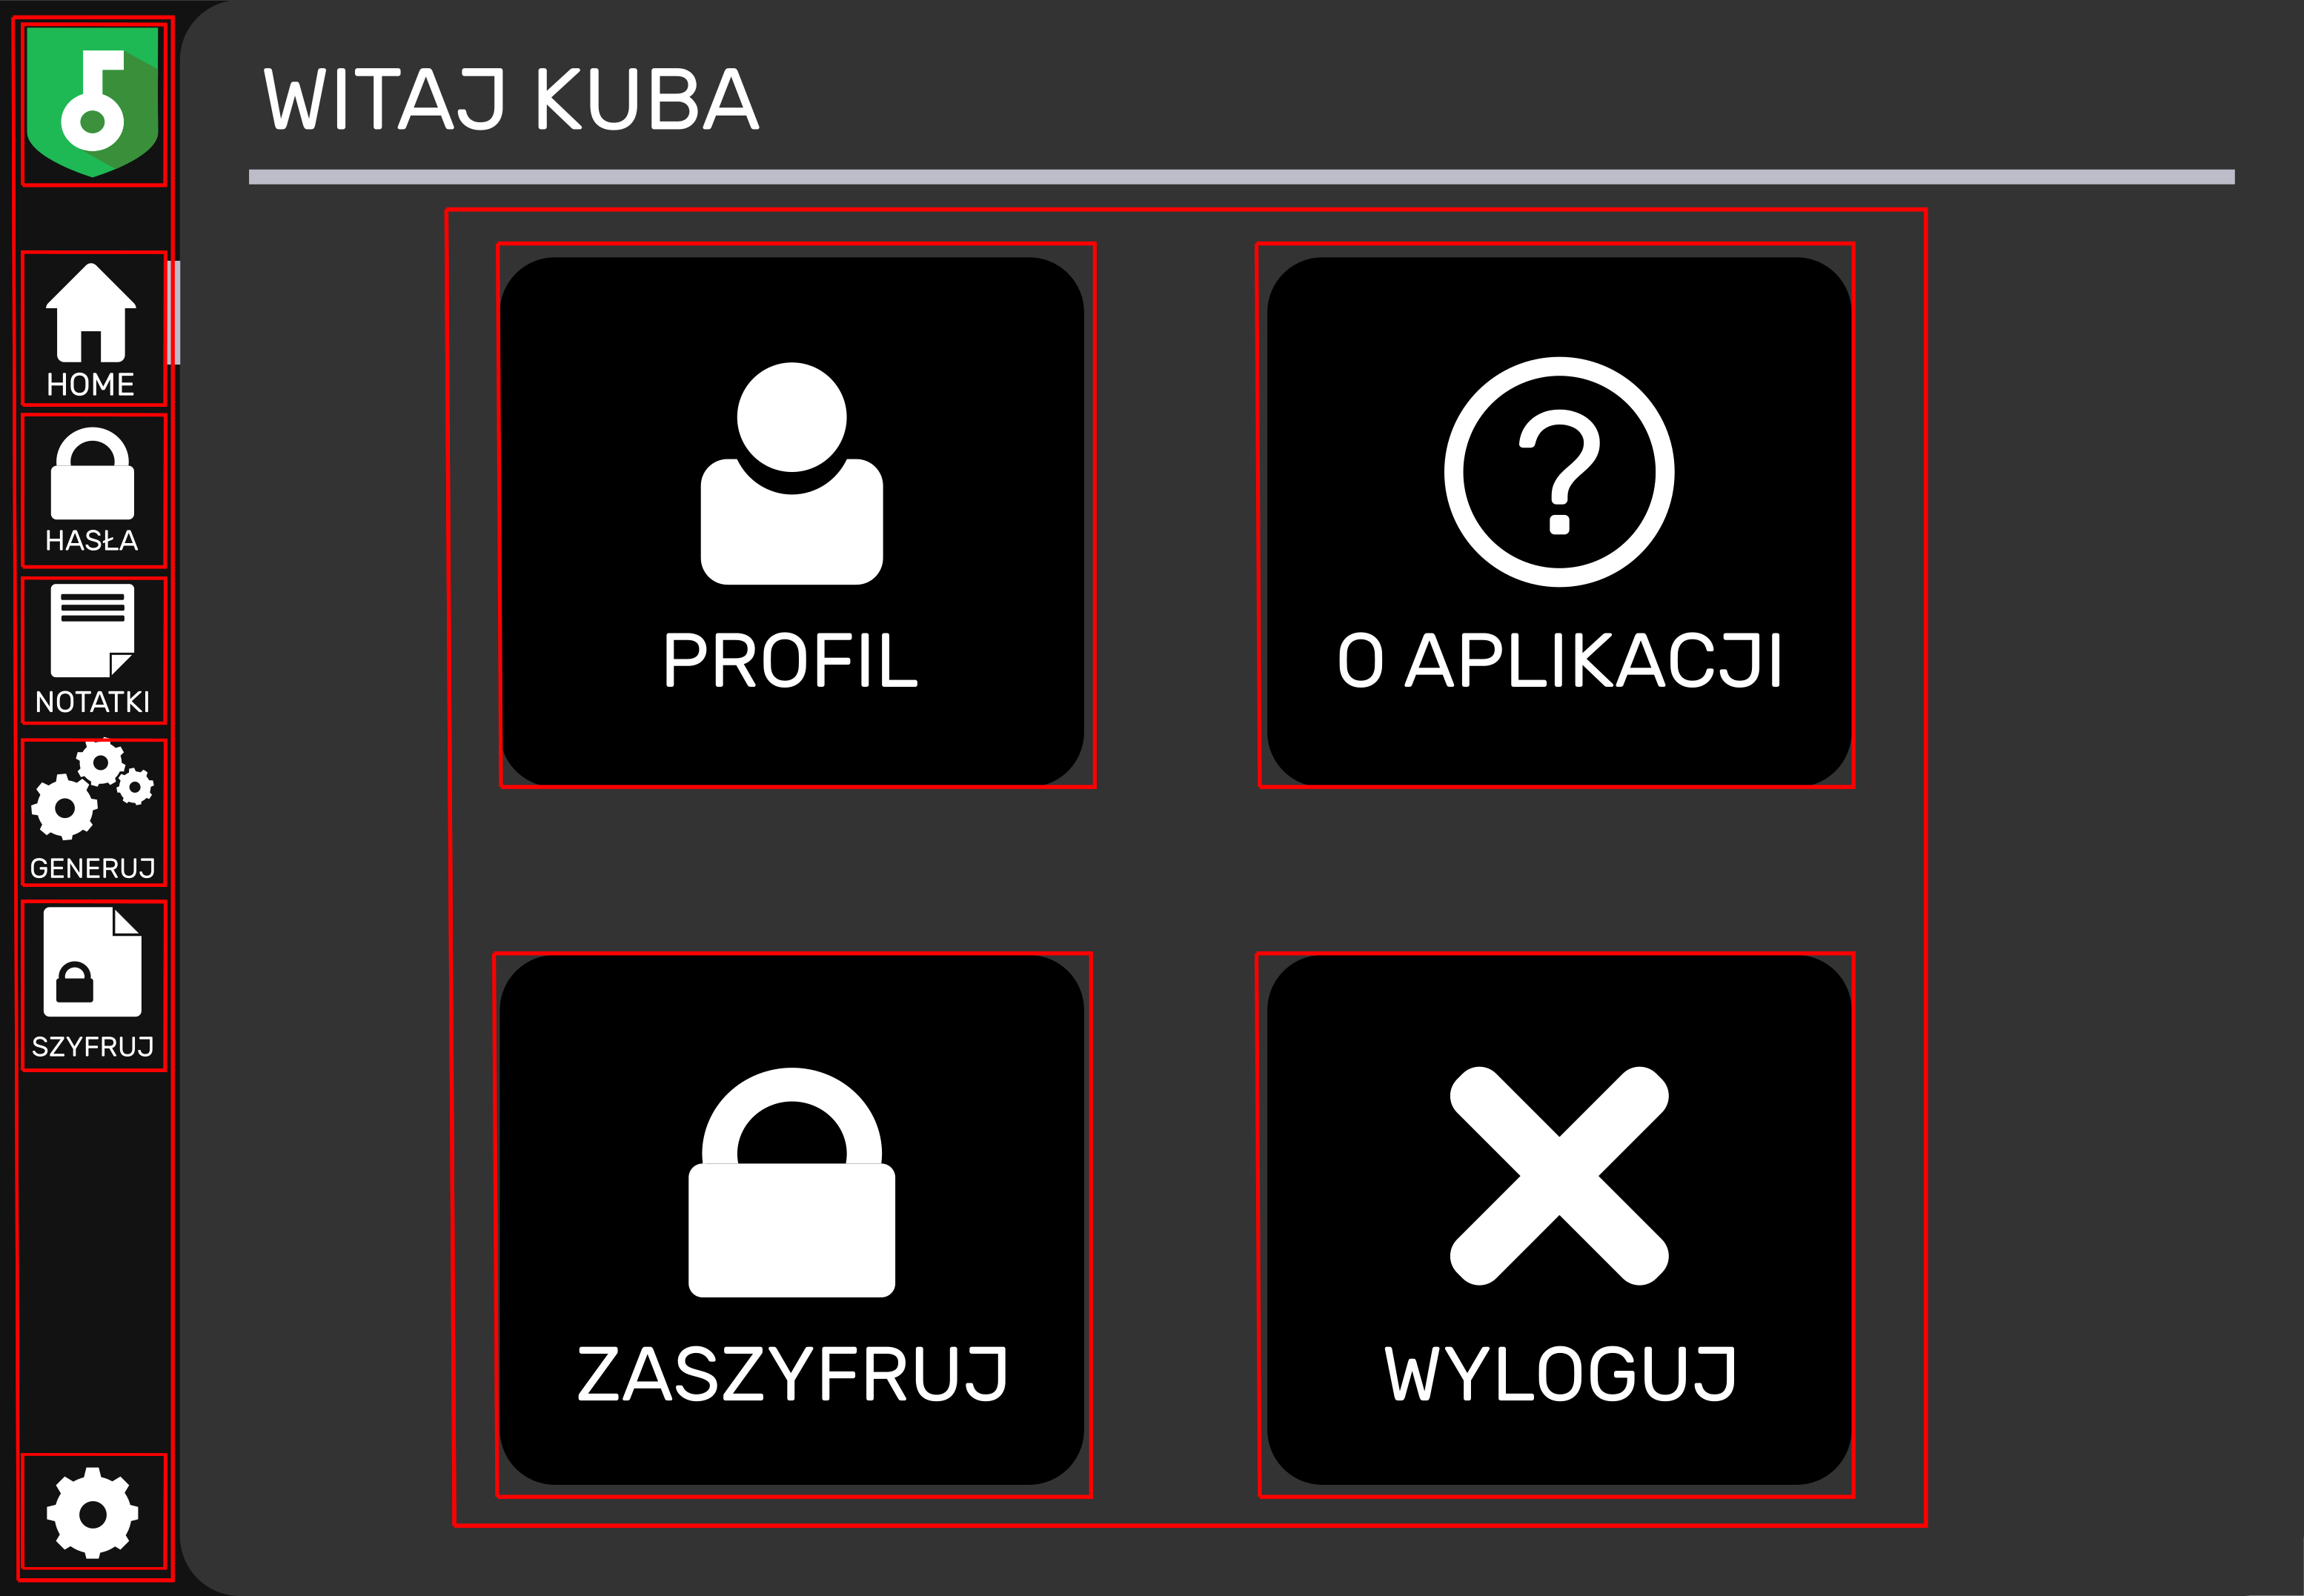
\includegraphics[width=1\textwidth]{img/ekran_po_zalogowaniu.png}
    \caption{Ekran startowy -- po zalogowaniu}
    \label{fig:startPo}
\end{figure}

\begin{figure}[H]
    \centering
    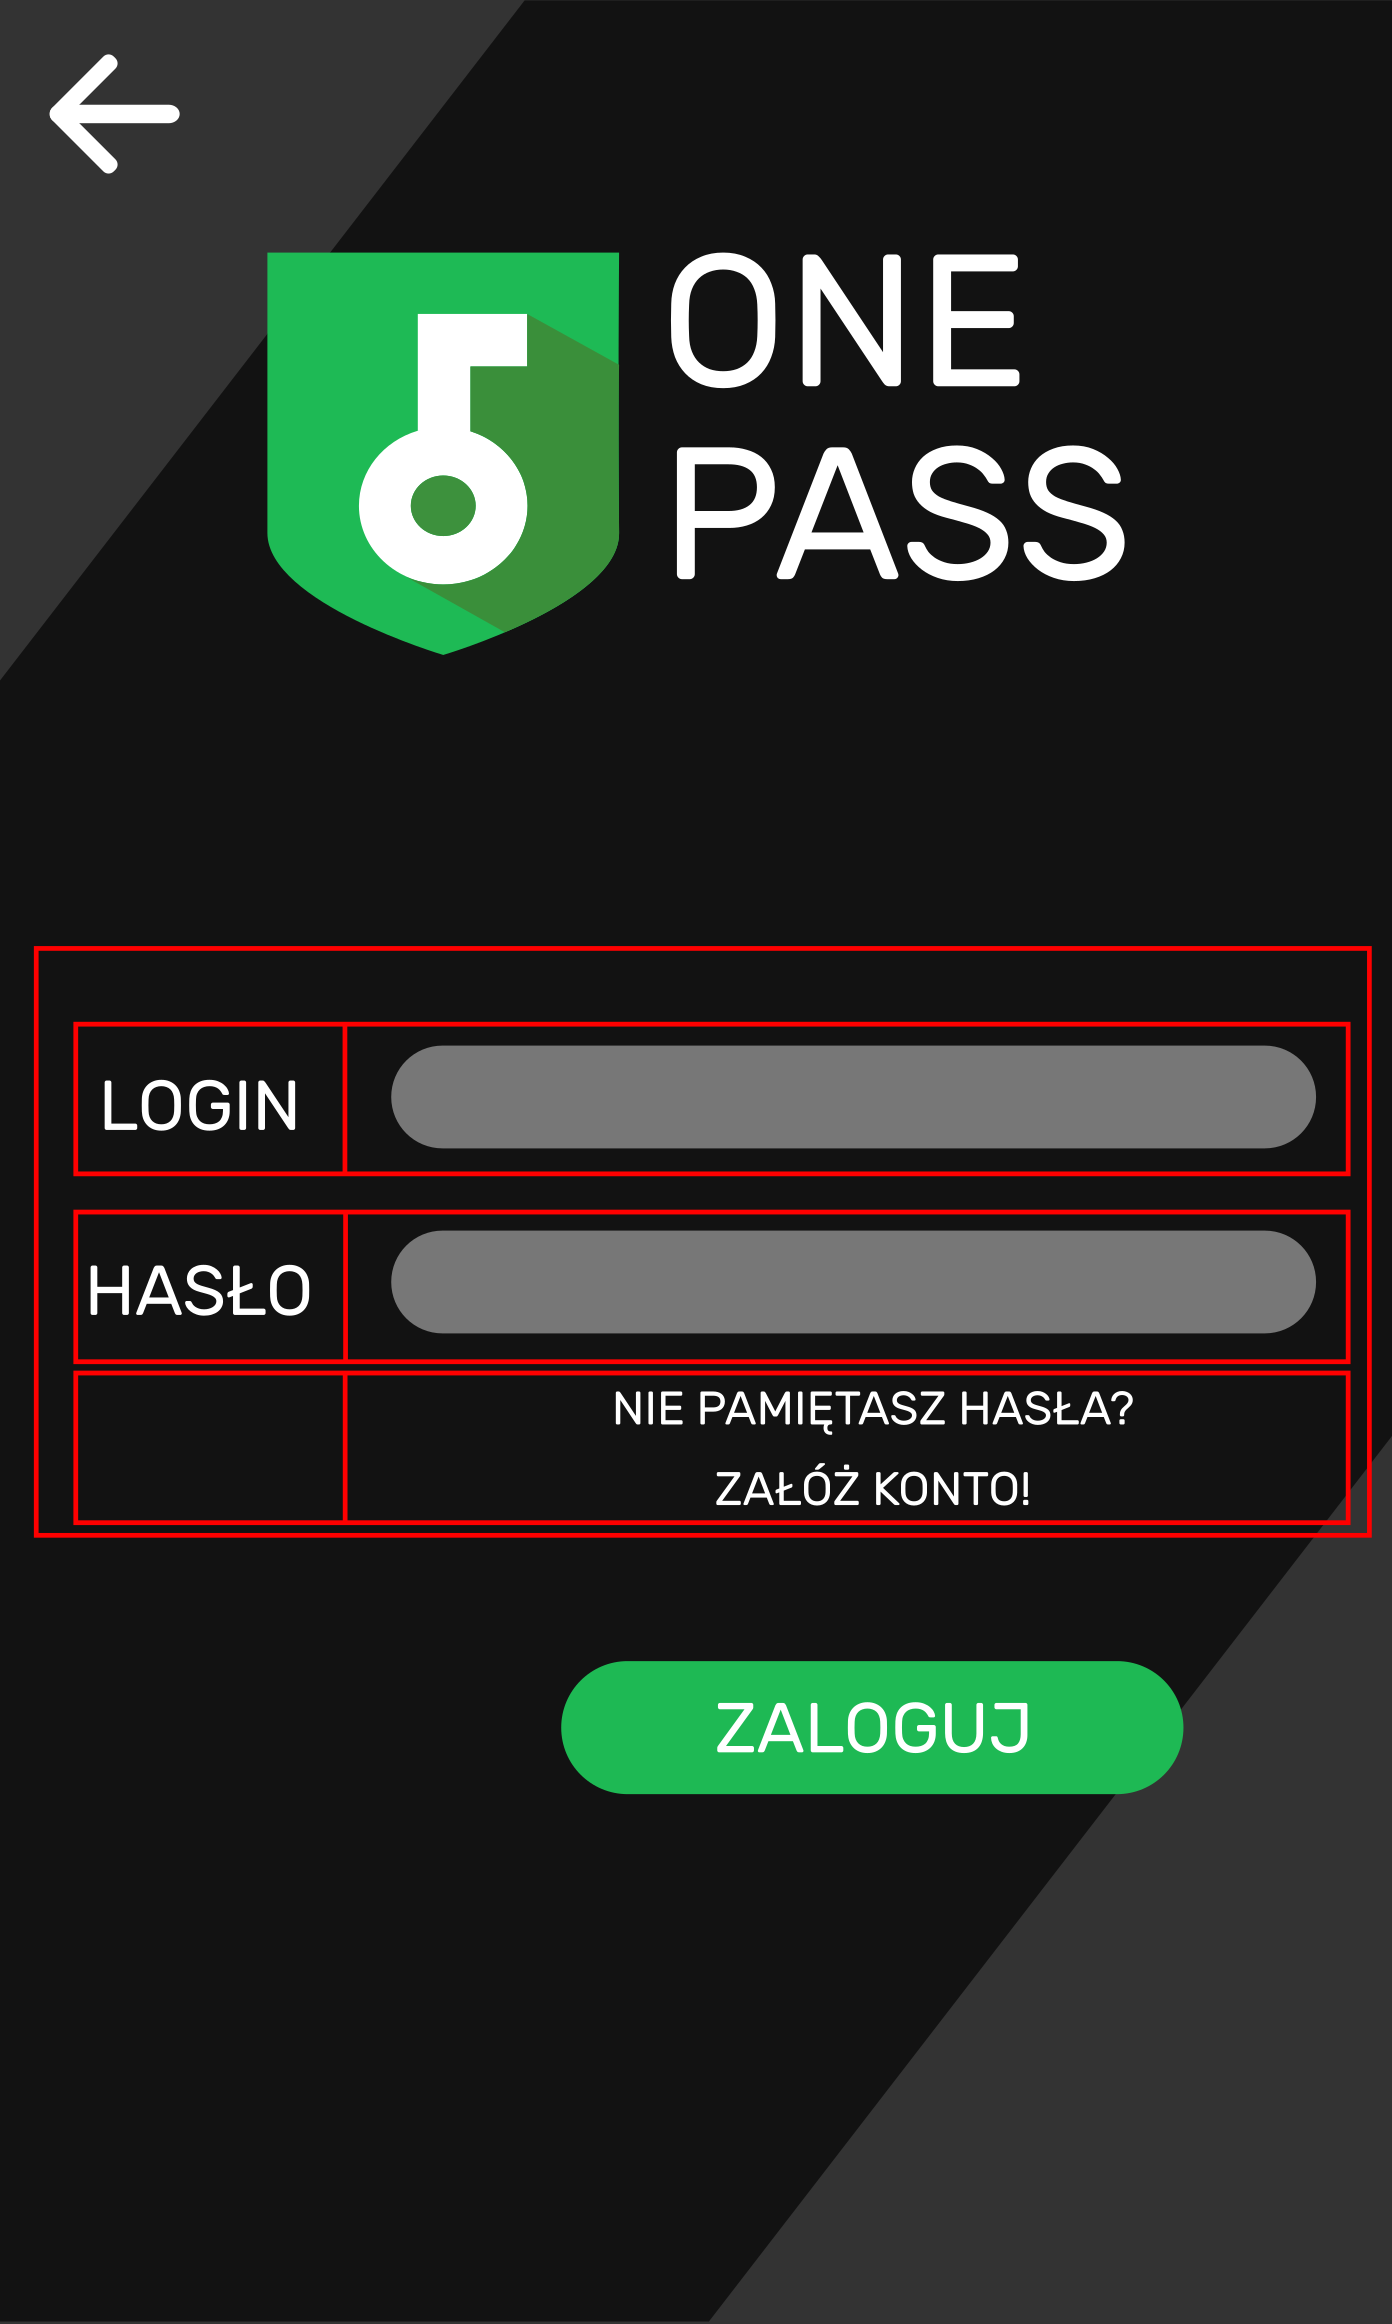
\includegraphics[height=1\textwidth]{img/ekran_logowania.png}
    \caption{Ekran logowania}
    \label{fig:logowanie}
\end{figure}

\begin{figure}[H]
    \centering
    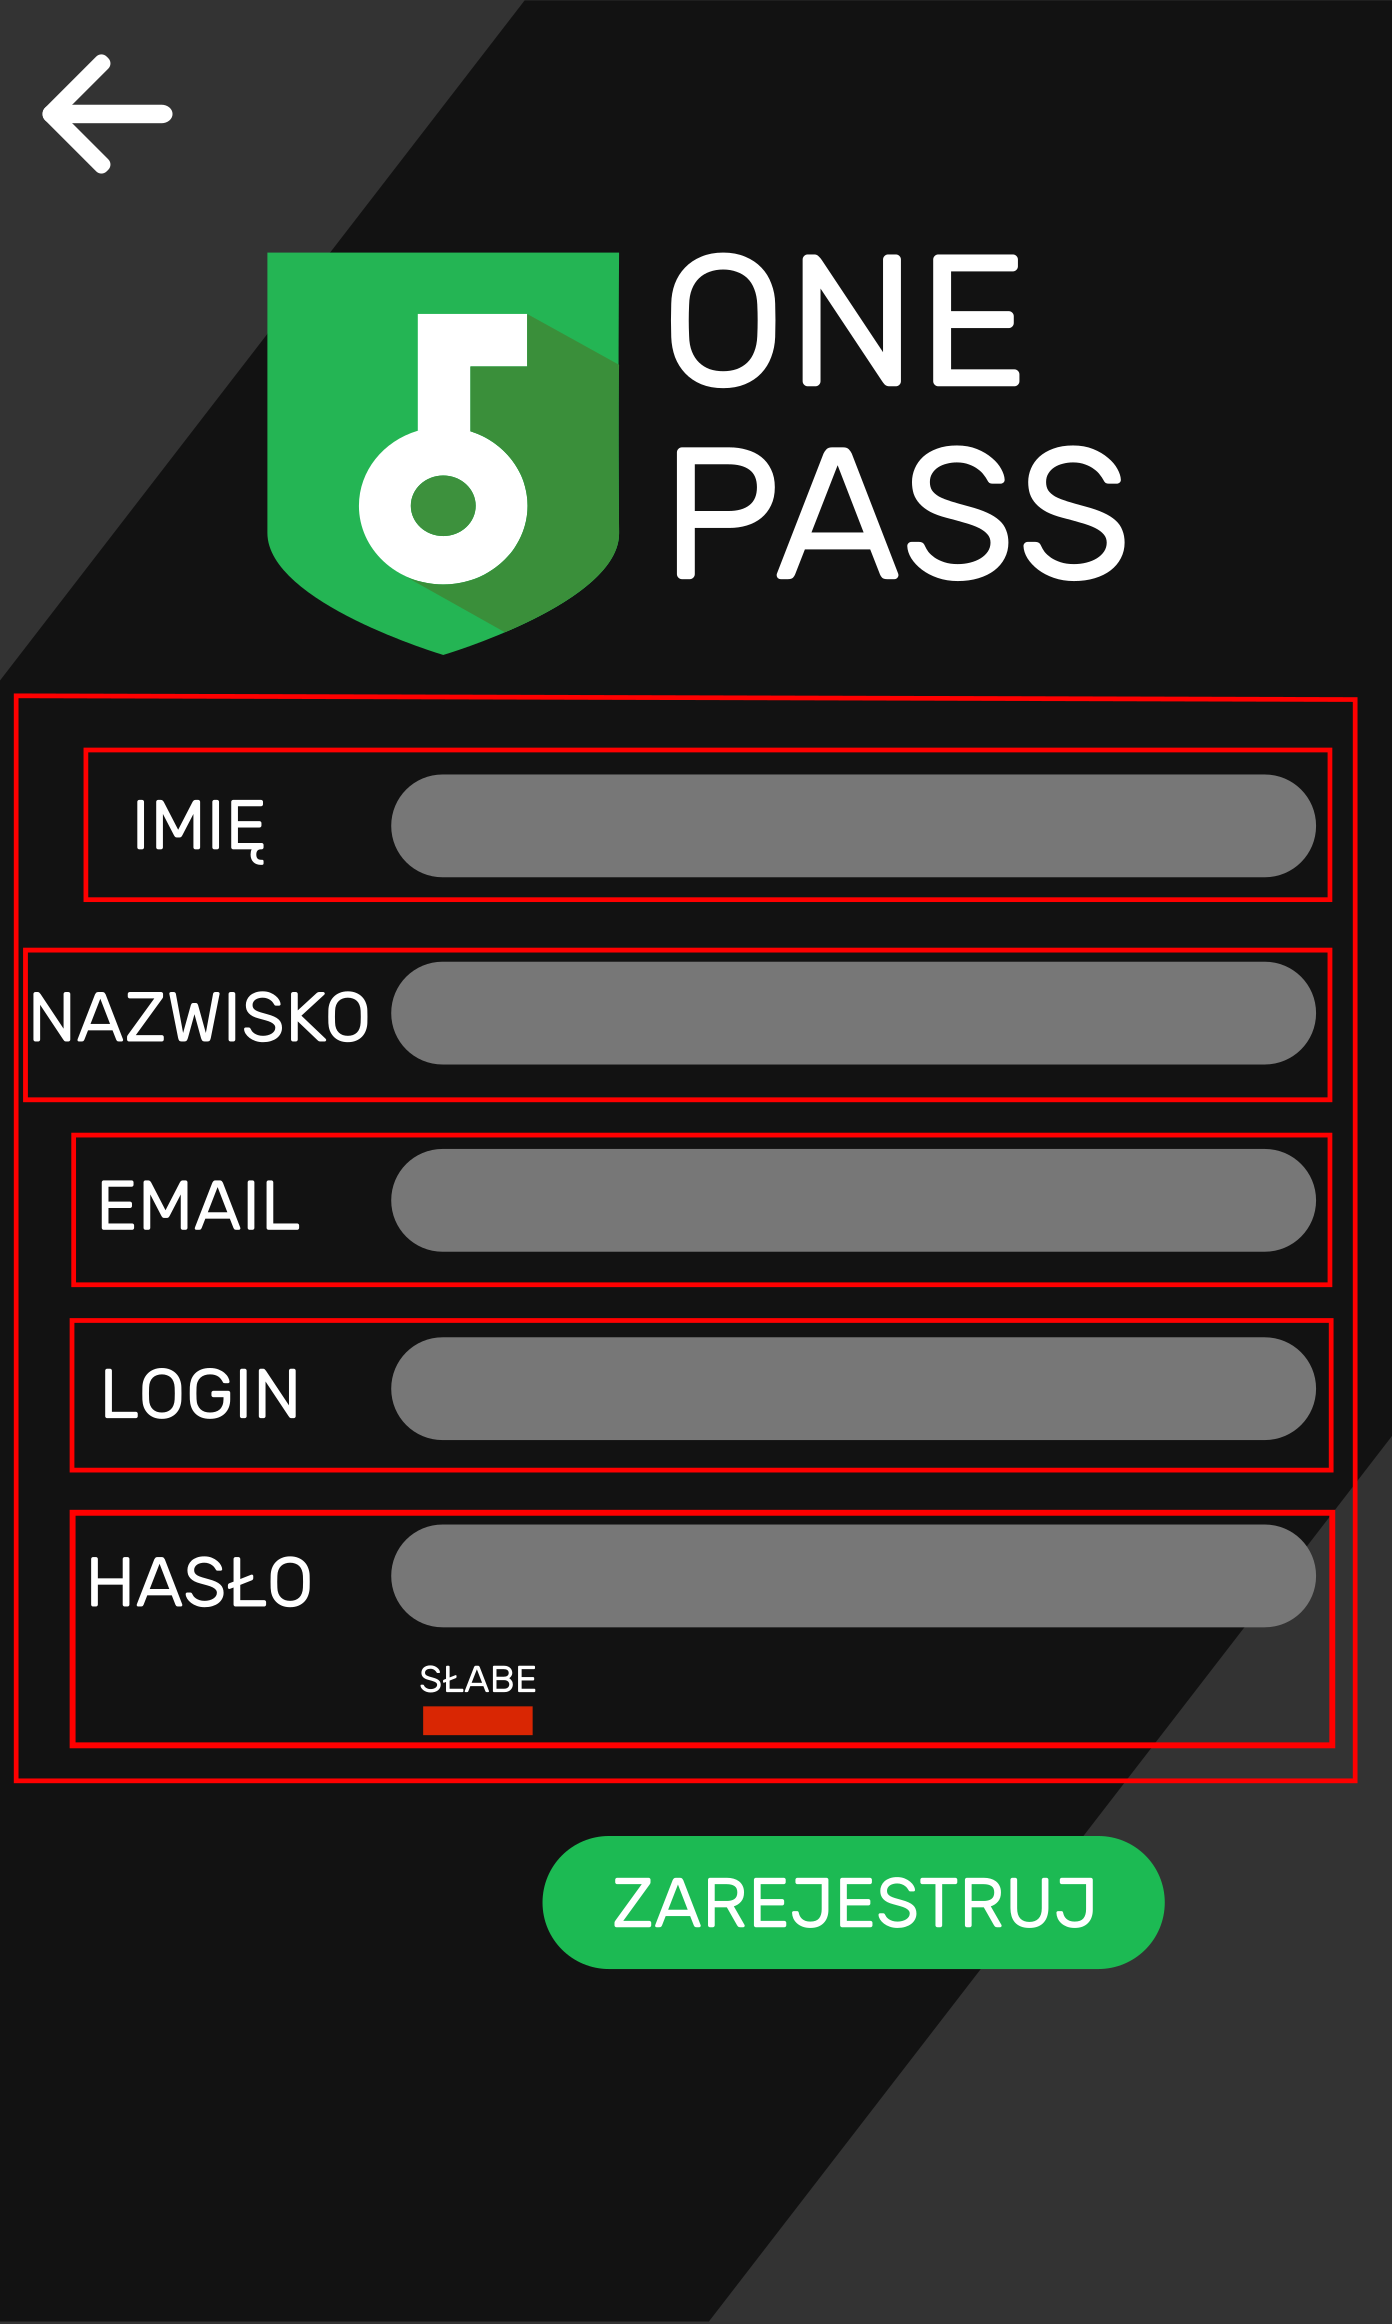
\includegraphics[height=1\textwidth]{img/ekran_rej.png}
    \caption{Ekran rejestracji}
    \label{fig:rejestracja}
\end{figure}

\begin{figure}[H]
    \centering
    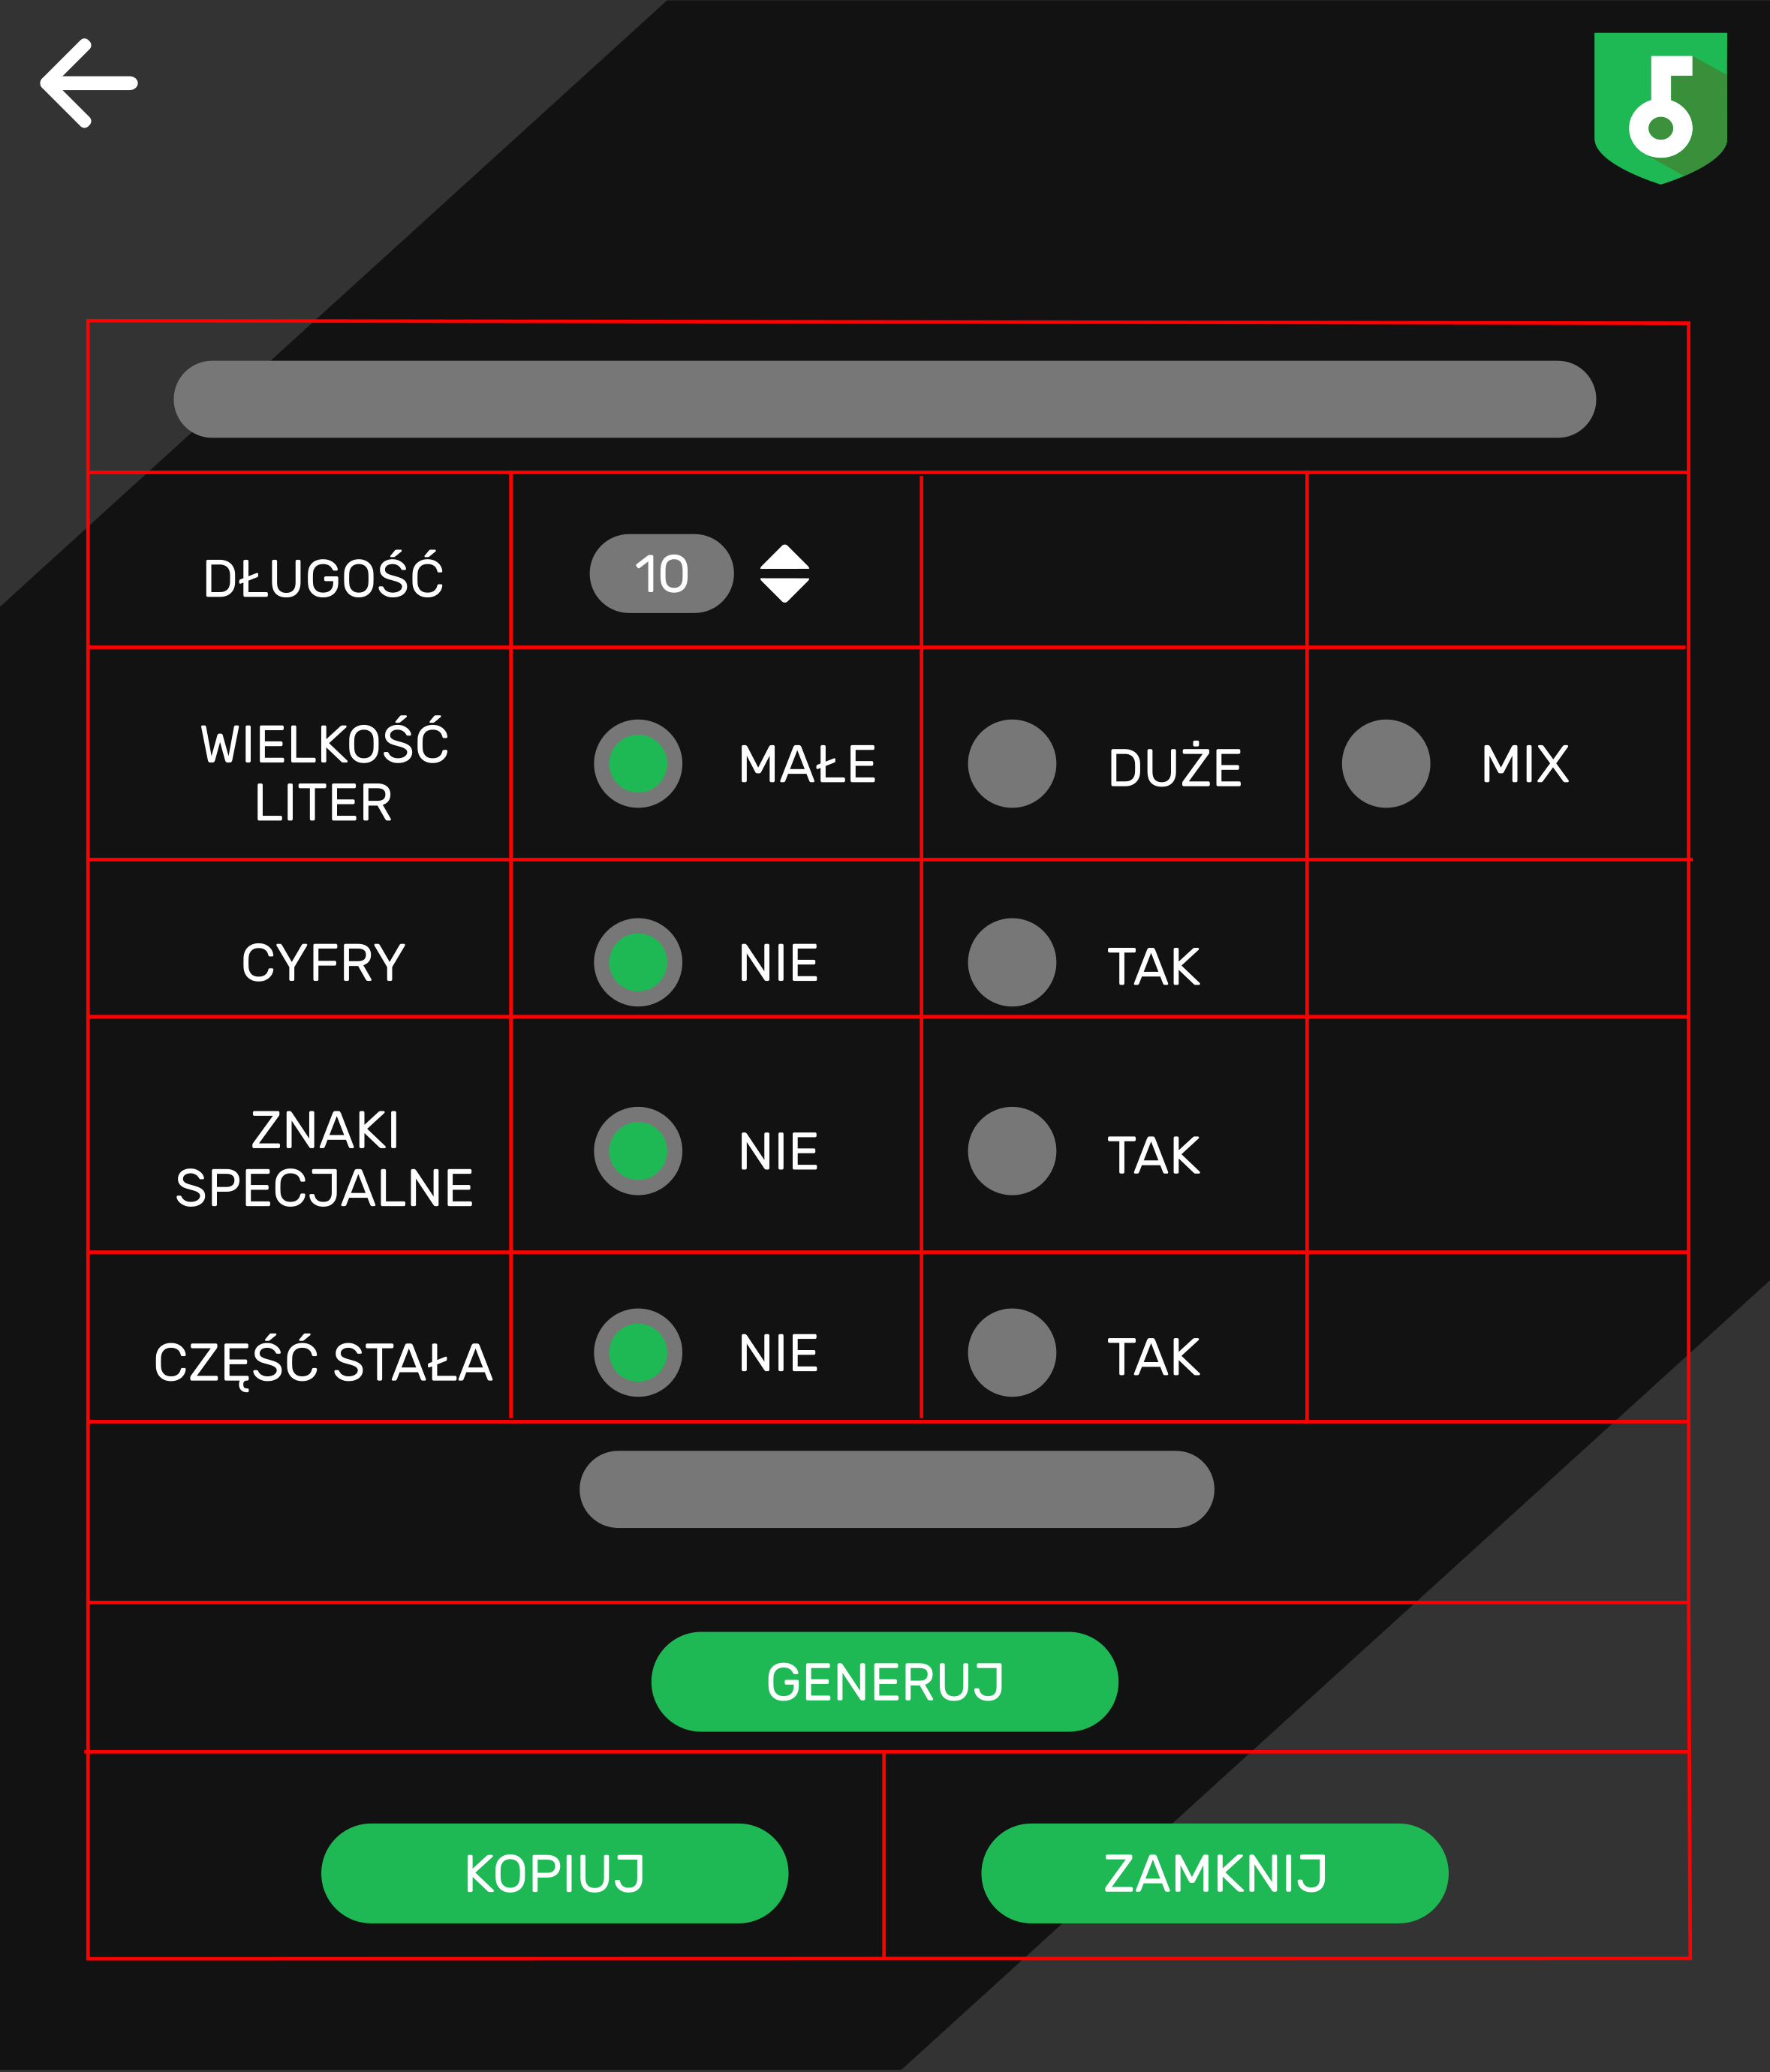
\includegraphics[height=1\textwidth]{img/ekran_generacji.png}
    \caption{Ekran generowania haseł}
    \label{fig:profil}
\end{figure}

\begin{figure}[H]
    \centering
    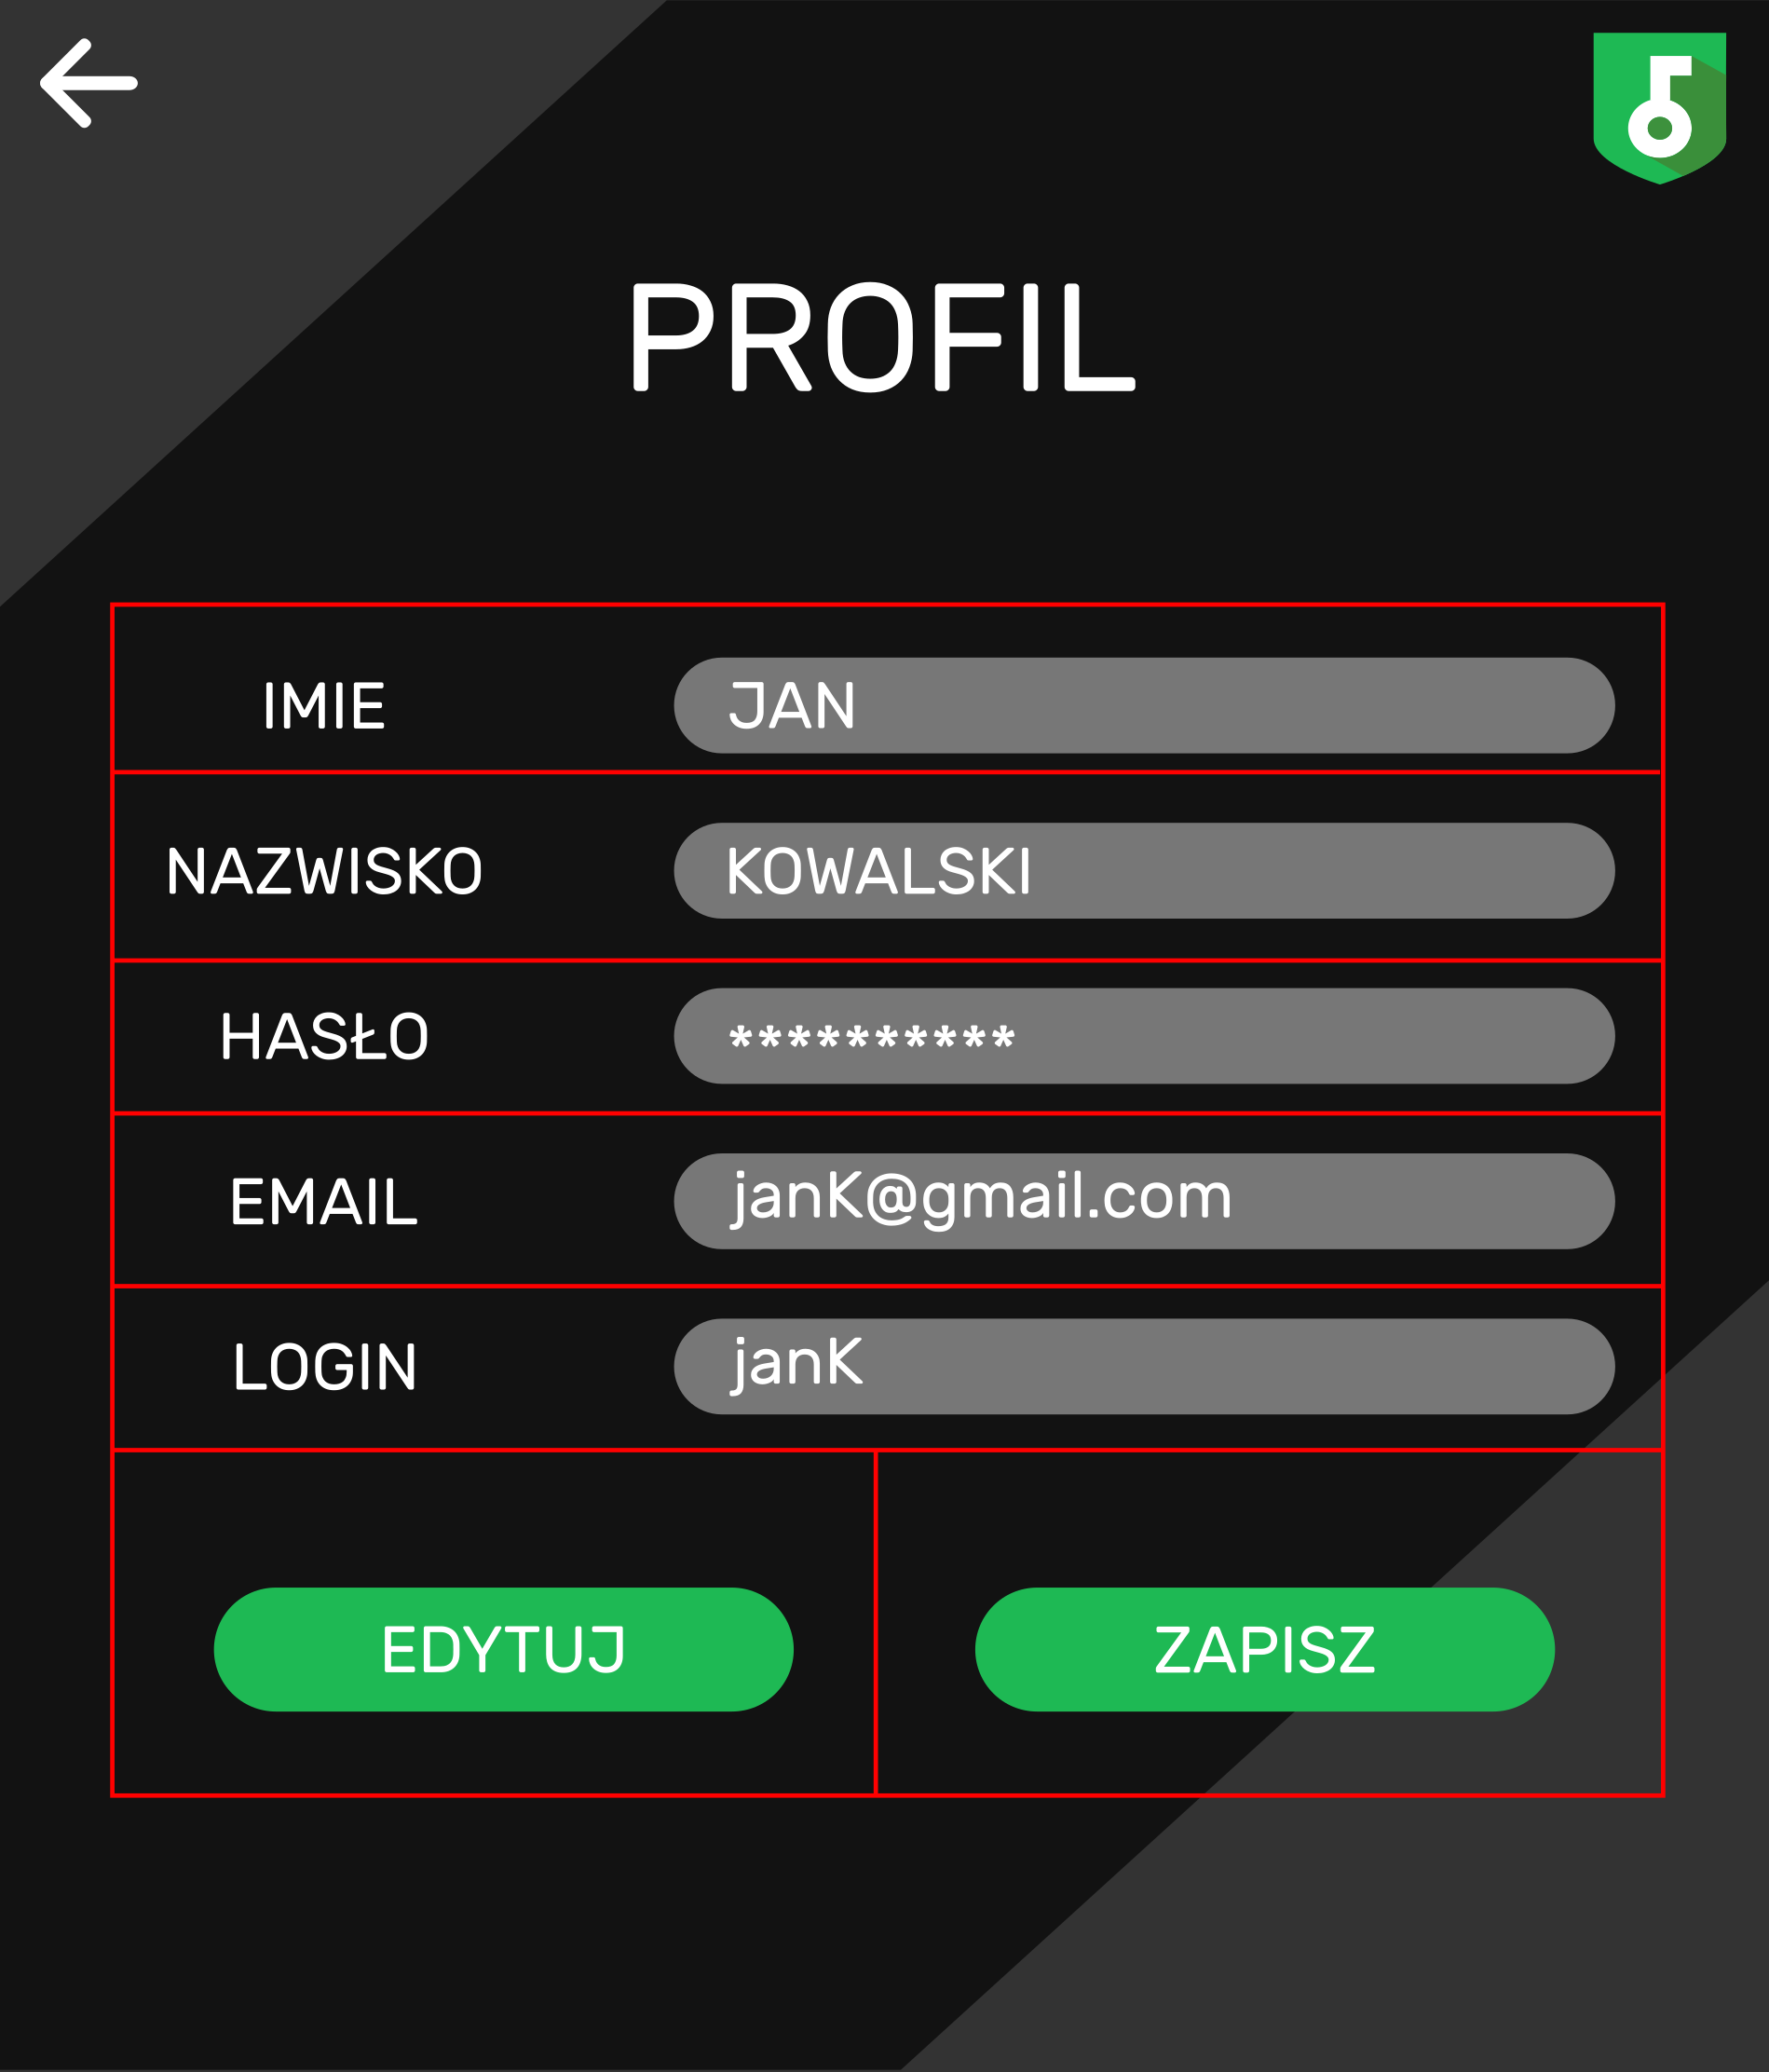
\includegraphics[height=1\textwidth]{img/ekran_profilu.png}
    \caption{Ekran informacji o profilu}
    \label{fig:profil}
\end{figure}

\begin{figure}[H]
    \centering
    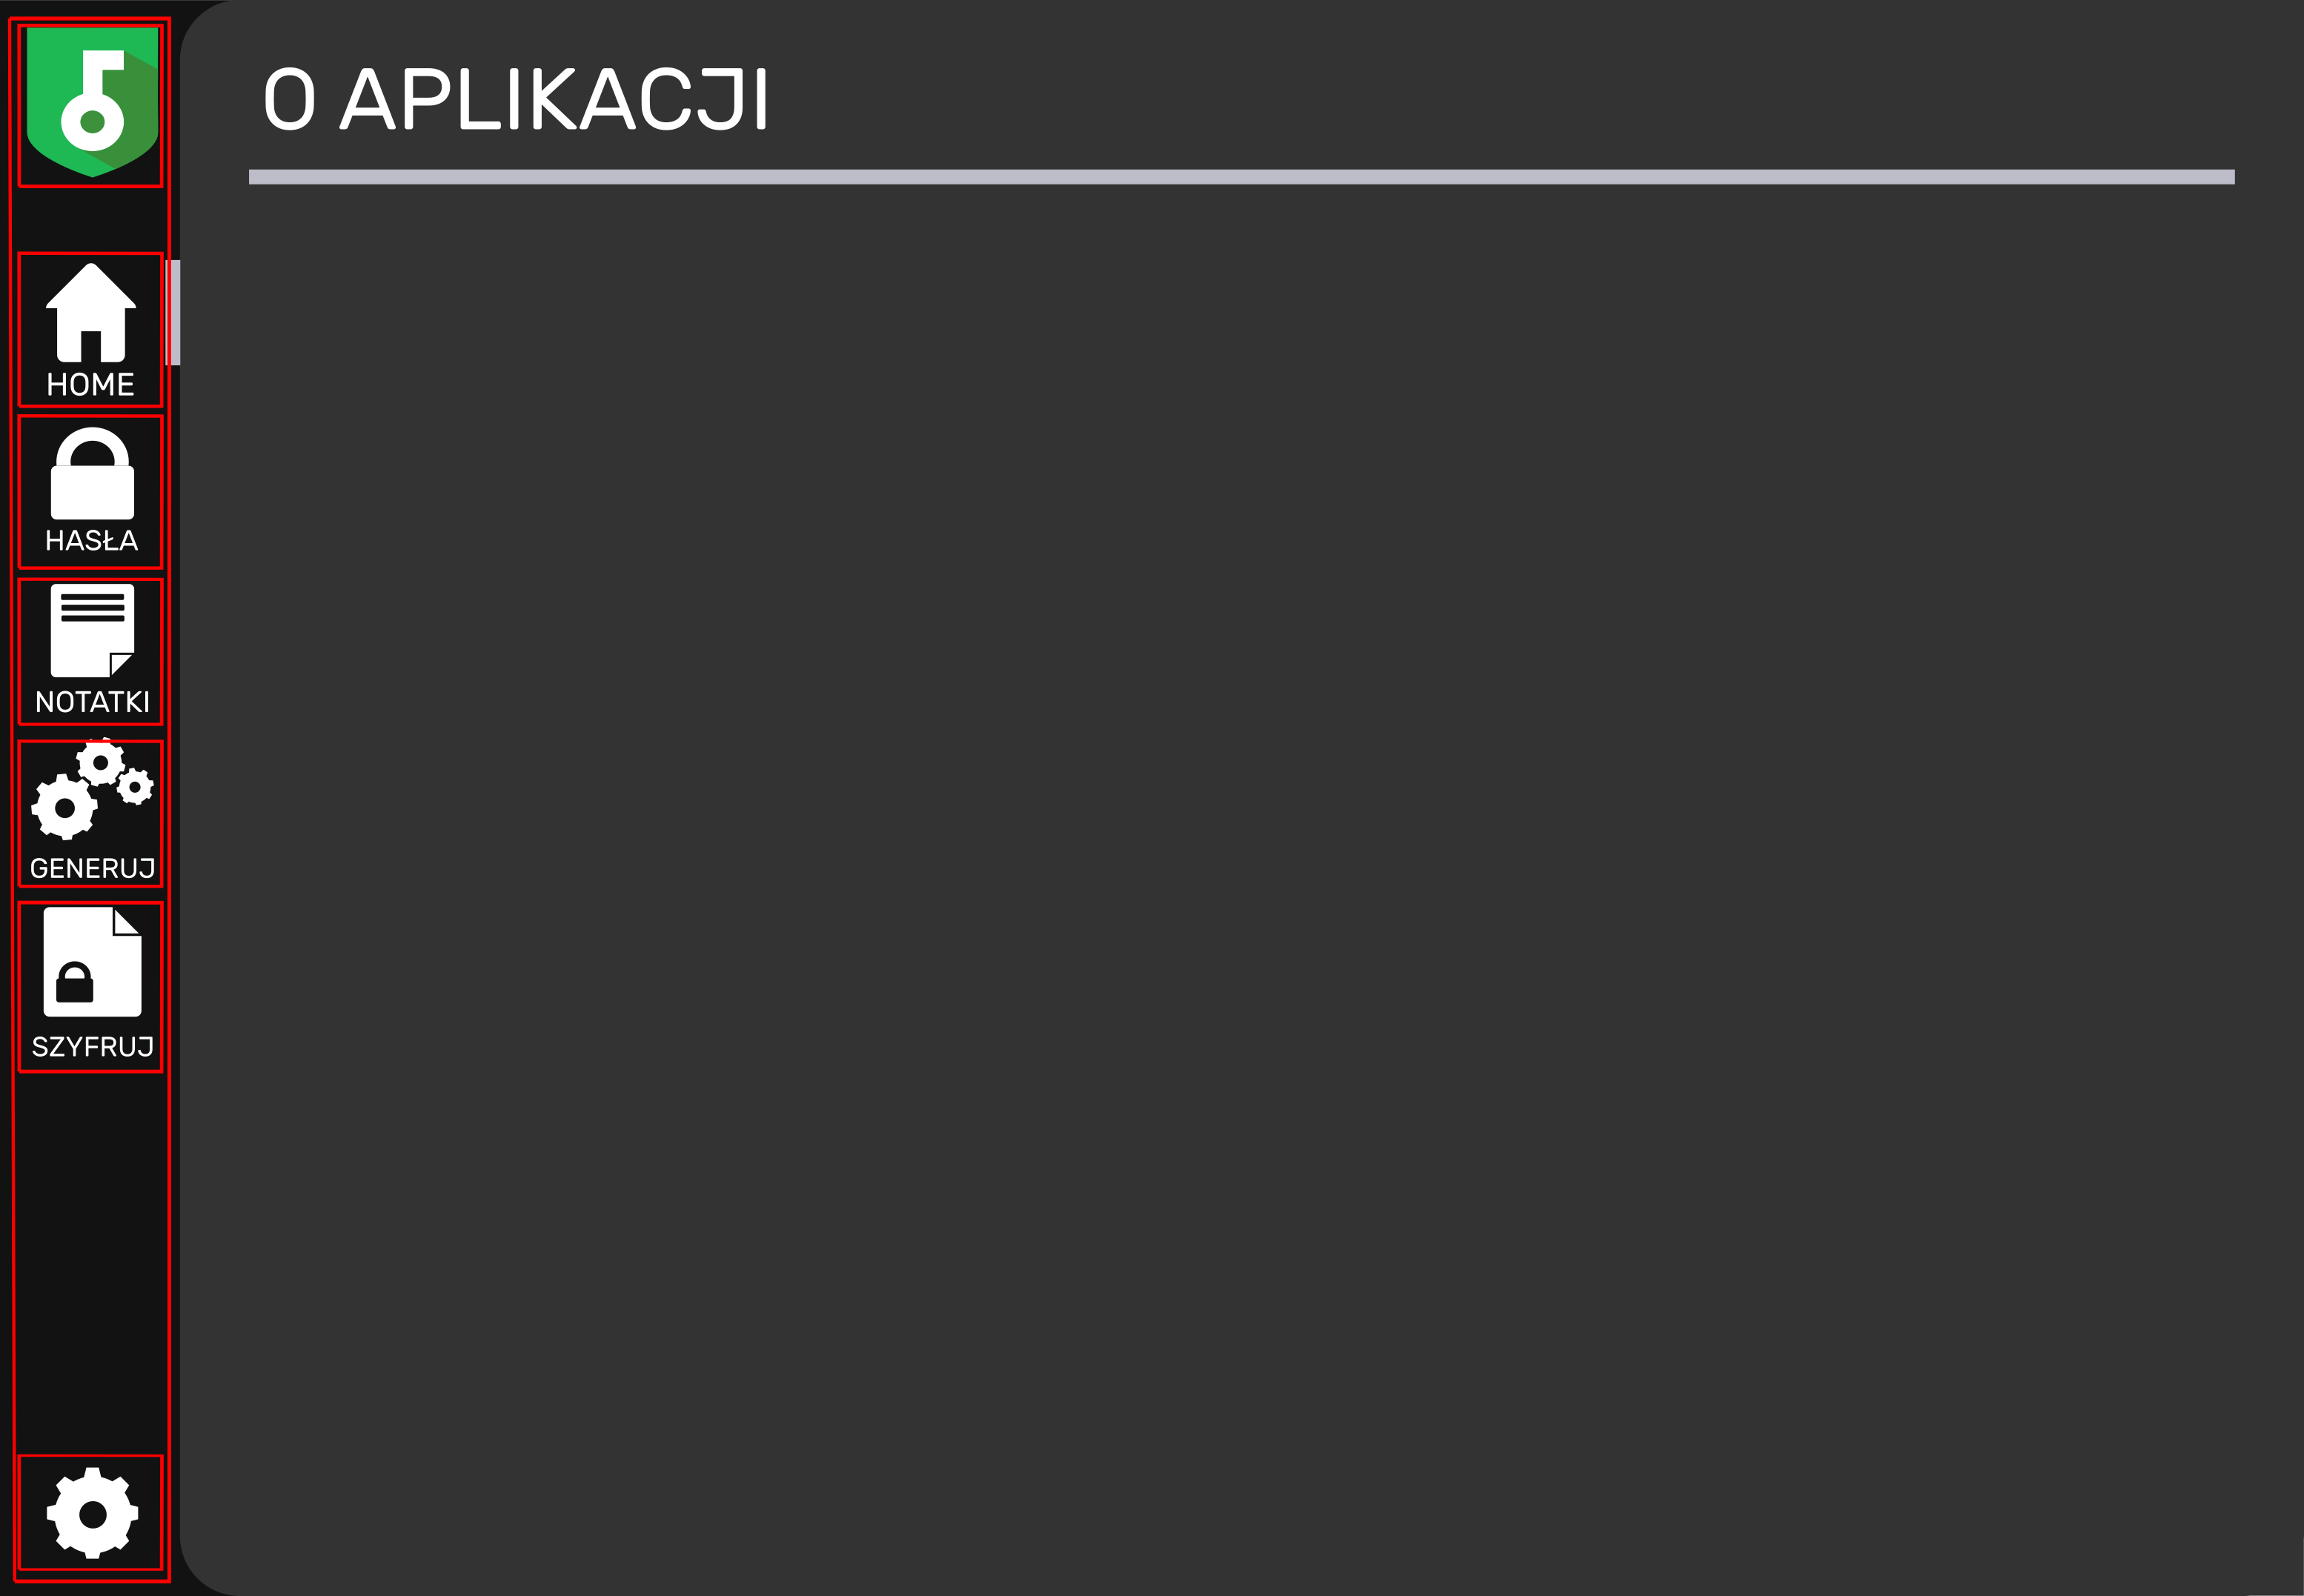
\includegraphics[width=1\textwidth]{img/ekarn_oapp.png}
    \caption{Ekran o aplikacji}
    \label{fig:oApp}
\end{figure}

\begin{figure}[H]
    \centering
    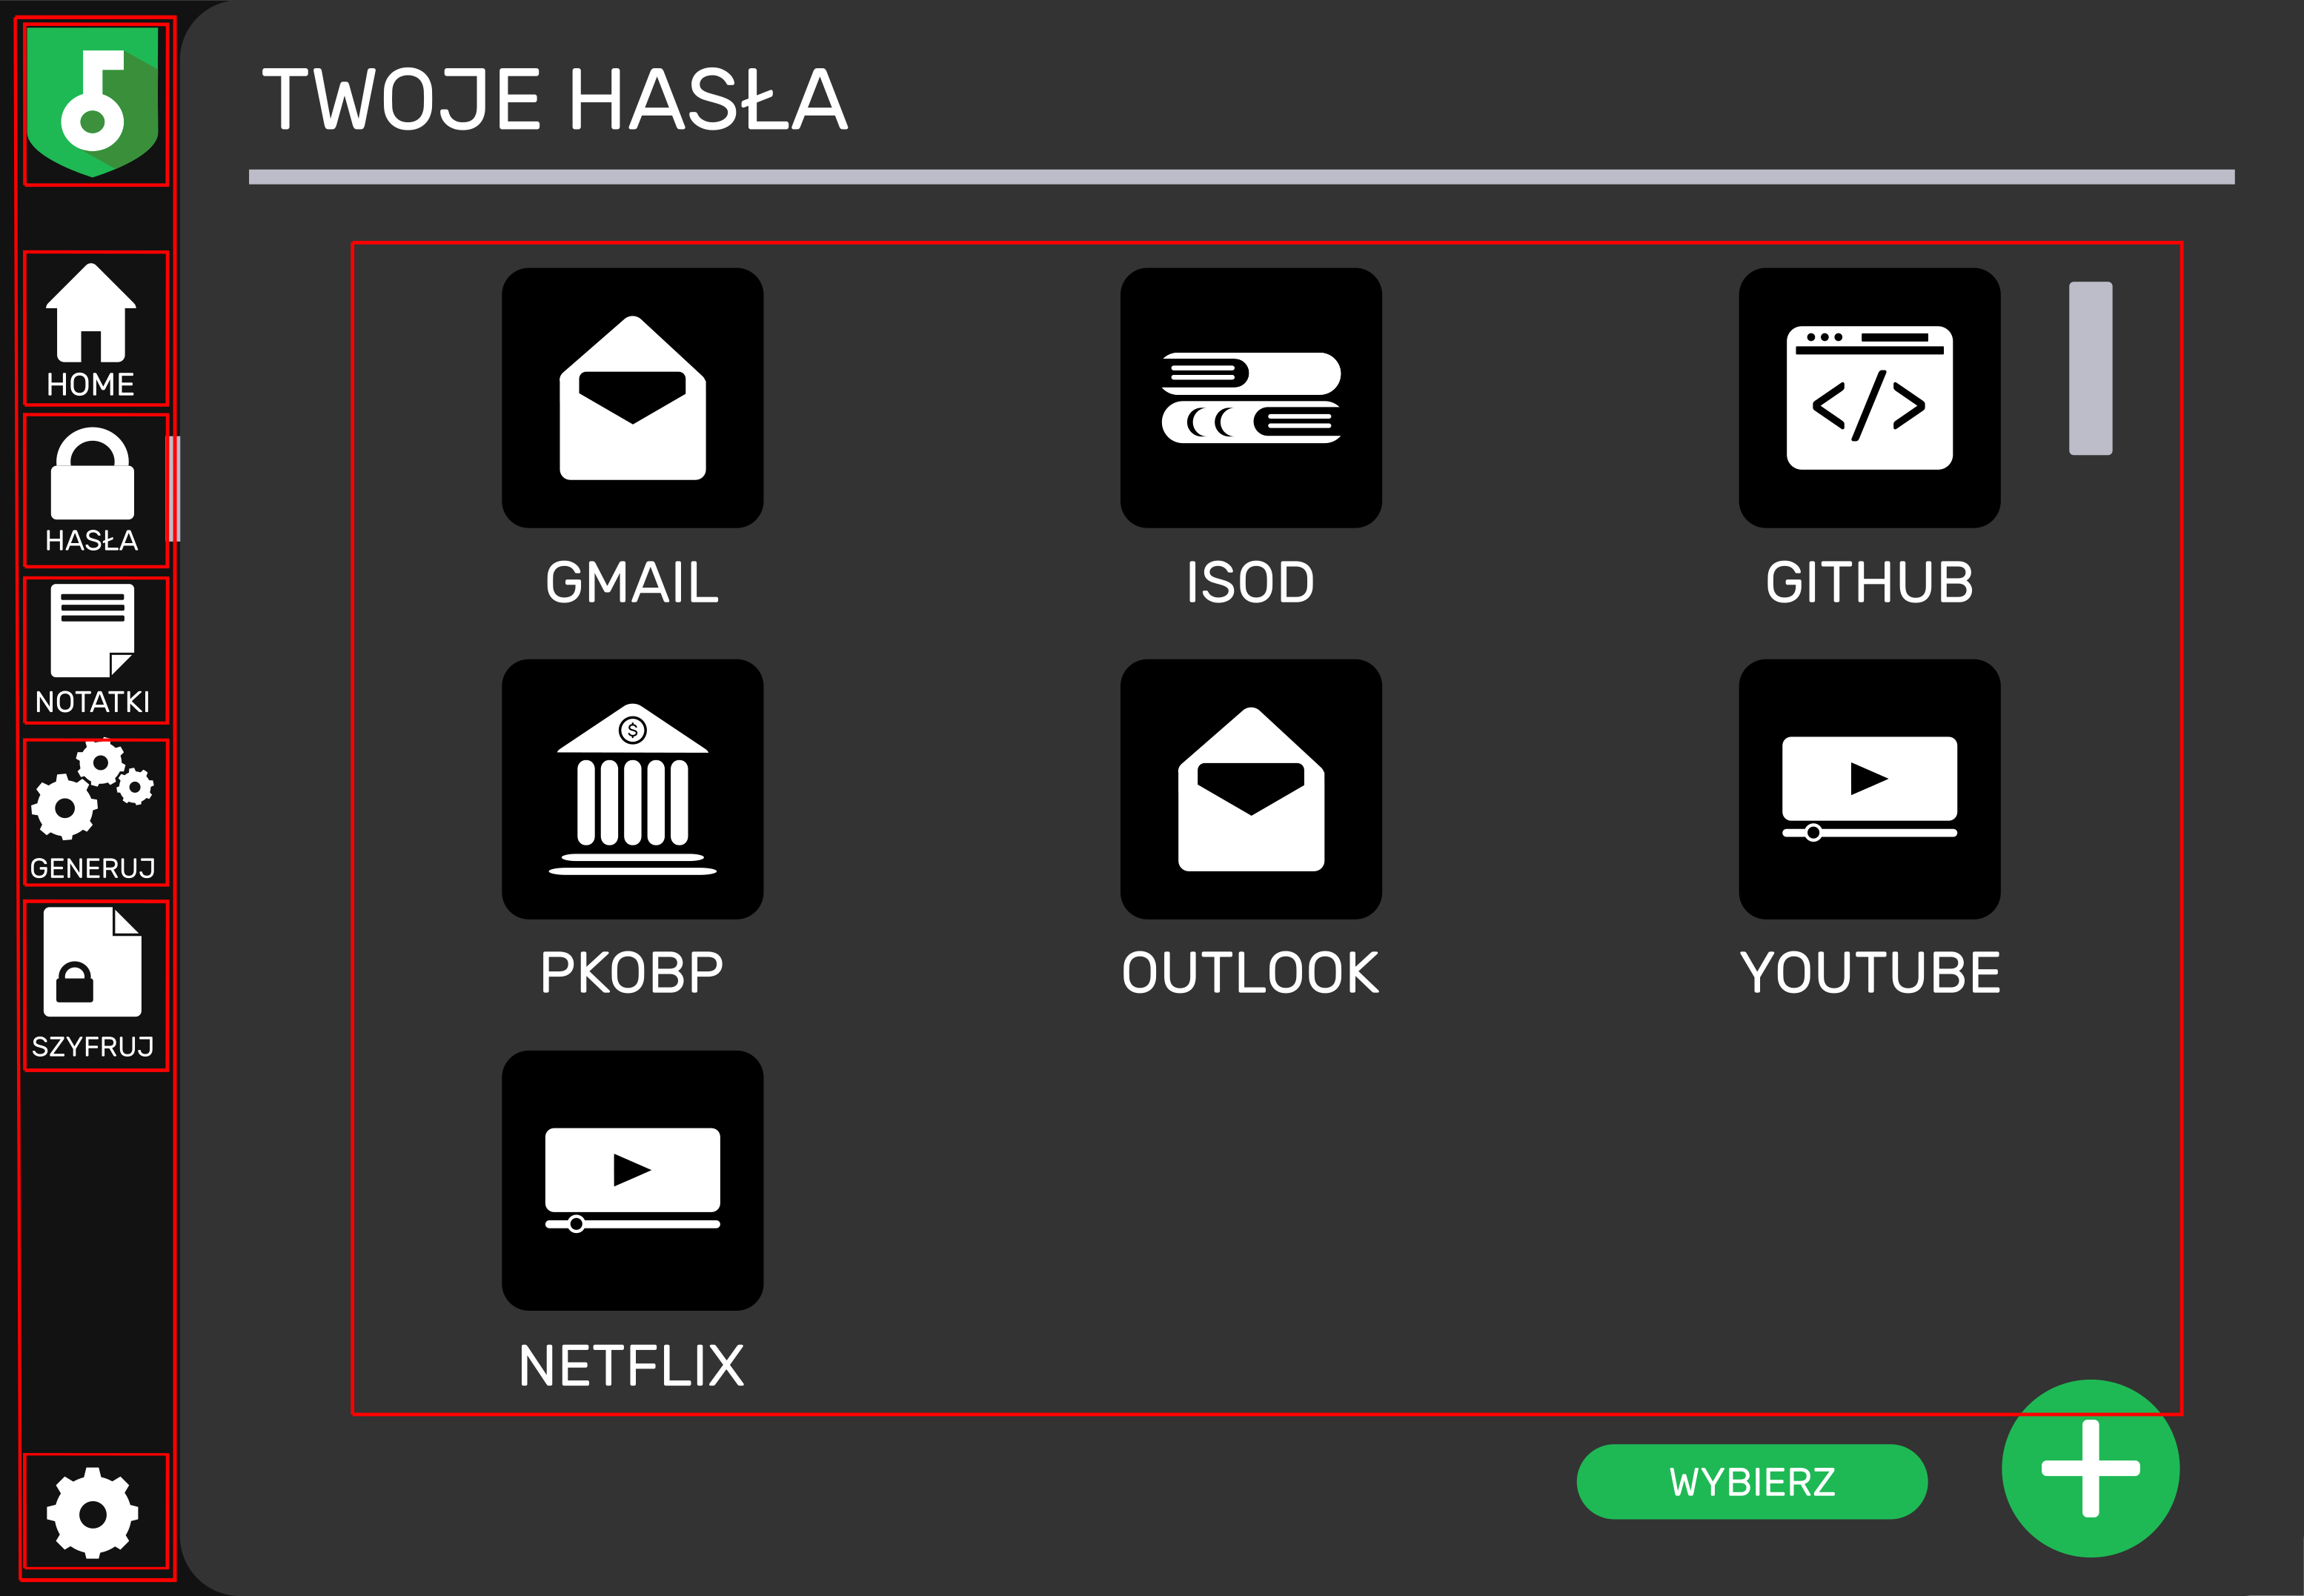
\includegraphics[width=1\textwidth]{img/ekran_hasel.png}
    \caption{Ekran haseł}
    \label{fig:hasla}
\end{figure}

\begin{figure}[H]
    \centering
    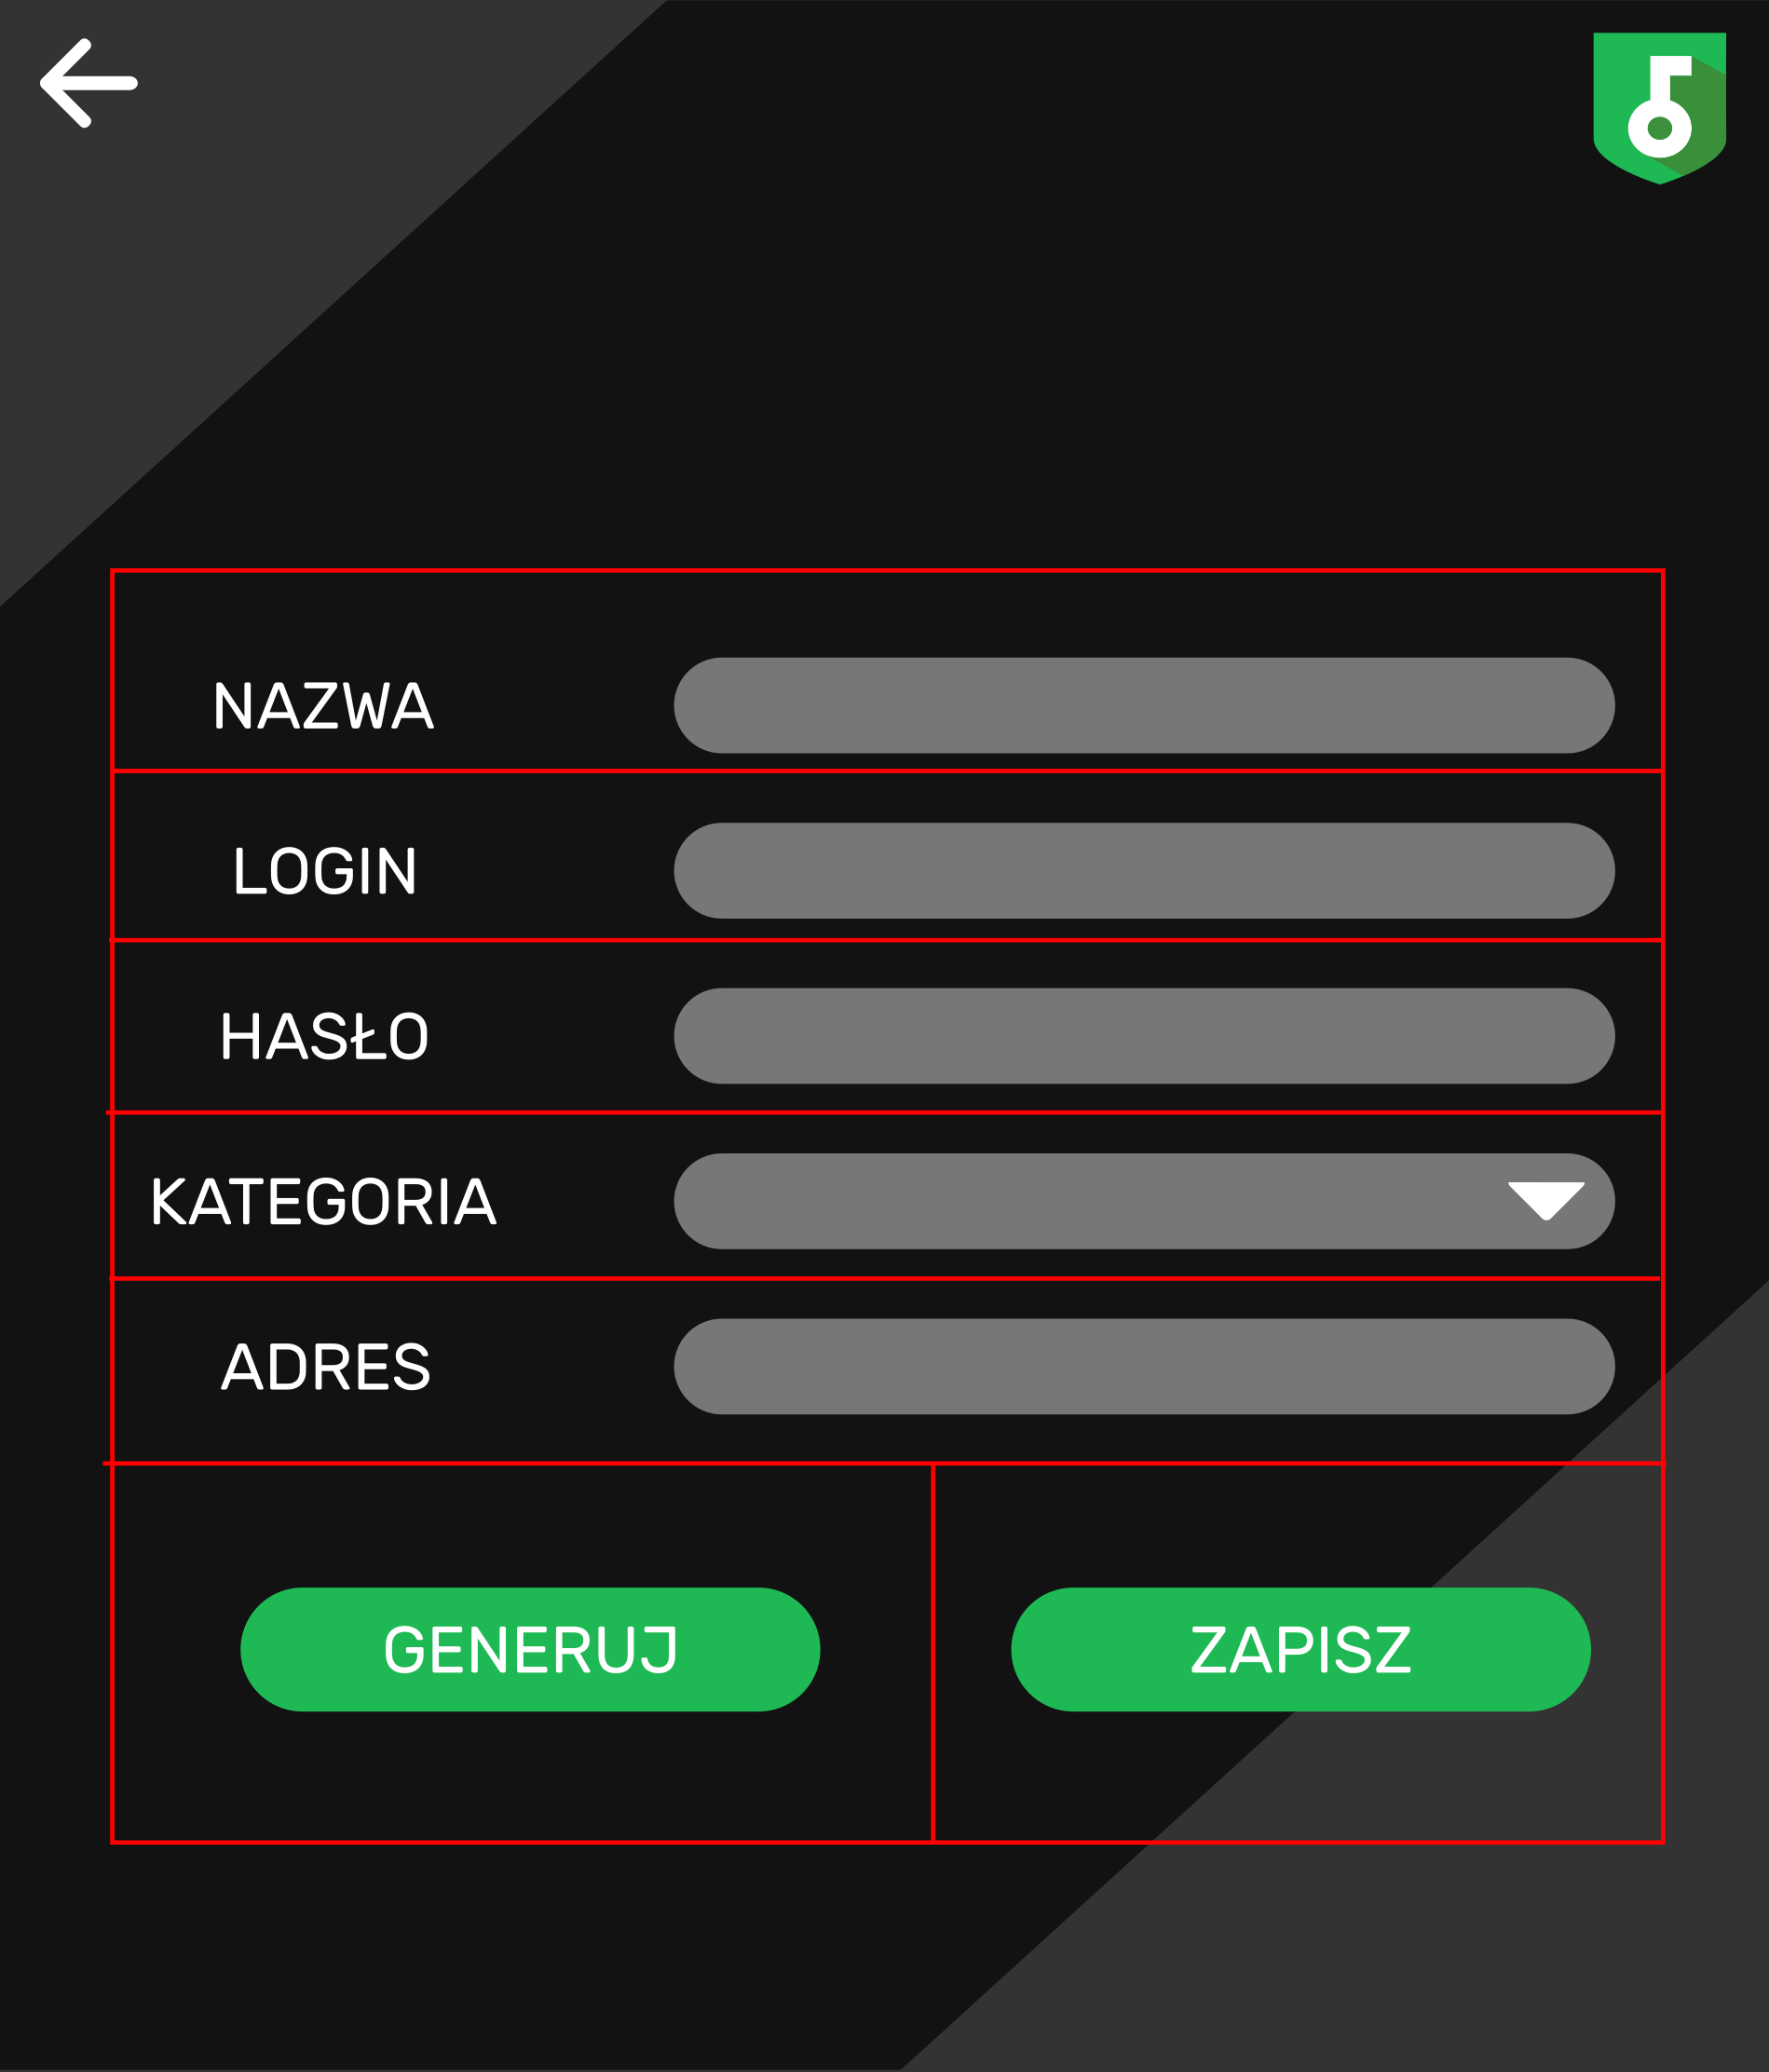
\includegraphics[height=1\textwidth]{img/ekran_dodania.png}
    \caption{Ekran dodawania obiektu}
    \label{fig:haslaDodanie}
\end{figure}

\begin{figure}[H]
    \centering
    \includegraphics[width=1\textwidth]{img/ekran_notatek.png}
    \caption{Ekran listy notatek}
    \label{fig:notatki}
\end{figure}

\begin{figure}[H]
    \centering
    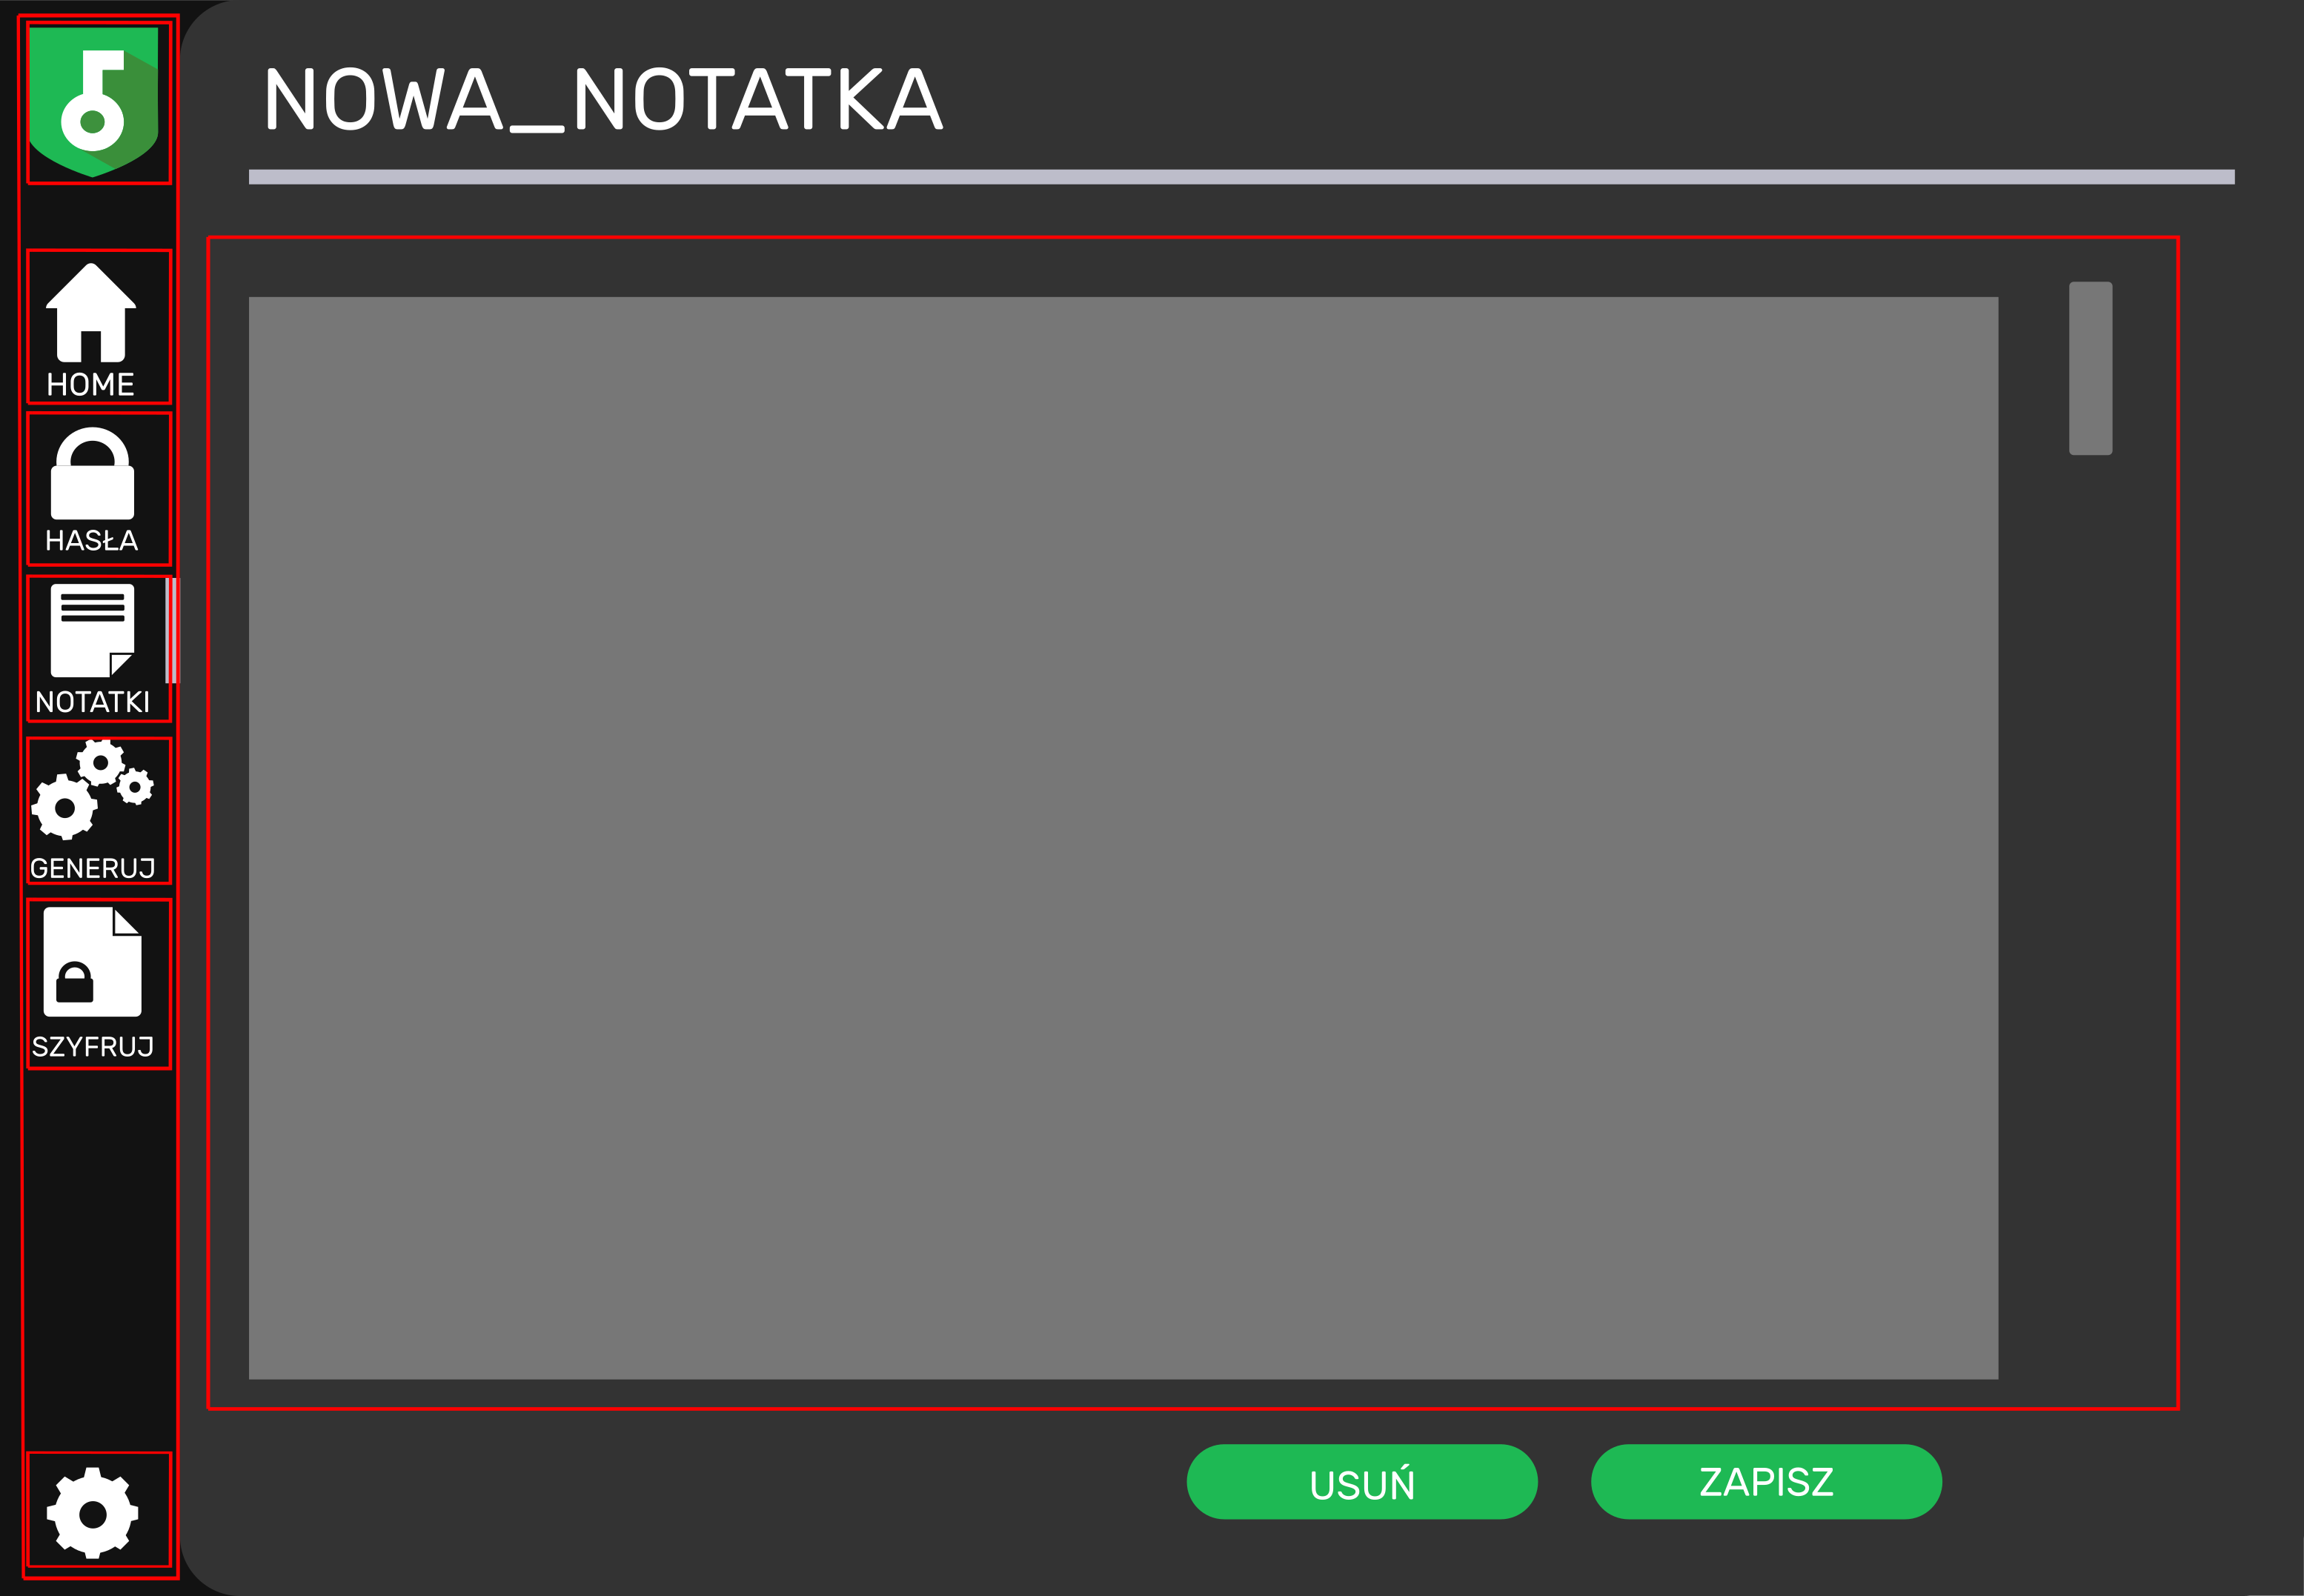
\includegraphics[width=1\textwidth]{img/ekran_nowej_not.png}
    \caption{Ekran dodawania lub edycji notatek}
    \label{fig:notatkNowe}
\end{figure}

\begin{figure}[H]
    \centering
    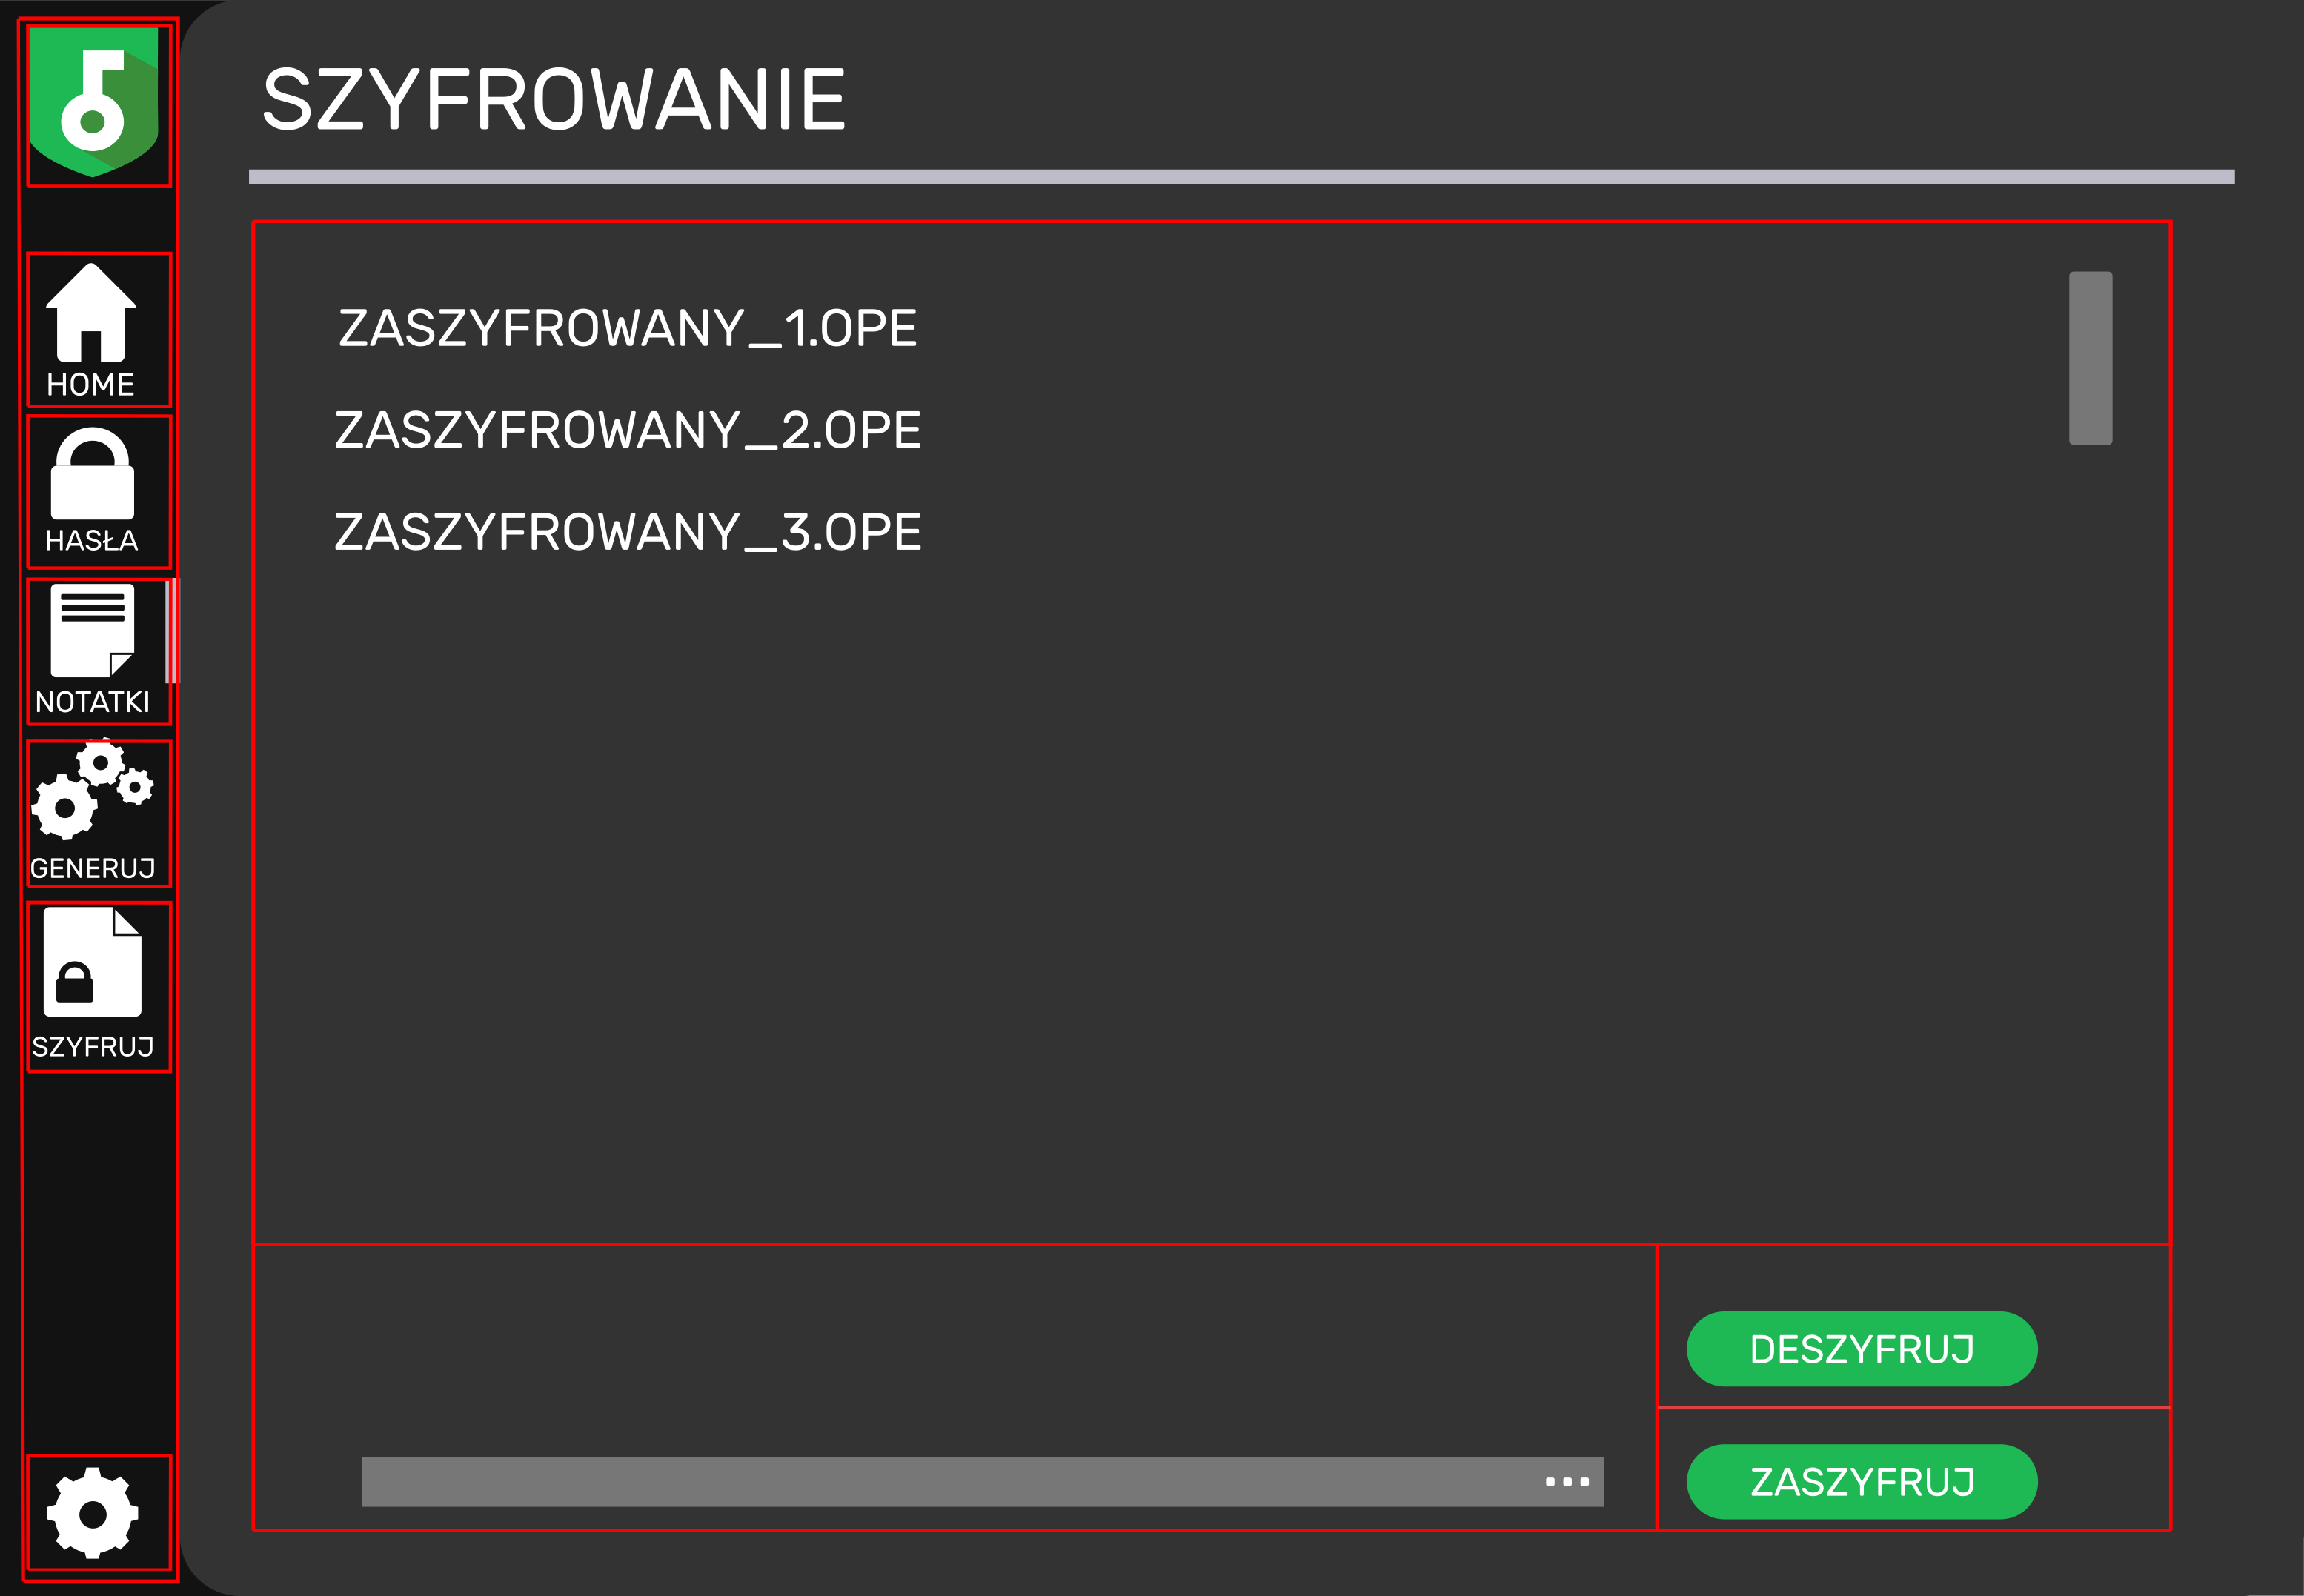
\includegraphics[width=1\textwidth]{img/ekran_szyfrowania.png}
    \caption{Ekran szyfrowania plików podanych przez użytkownika}
    \label{fig:szyfrowanie}
\end{figure}



\section{Testowanie}
\subsection{Użyte narzędzia}
Do przetestowania kodu użyje narzędzi z modułu \textit{unittest}. Natomiast GUI przetestuje ręcznie podczas tworzenia aplikacji. Dodatkowo gotowy program przetestuje sam używając go oraz przekaże go do testów znajomym.

\subsection{Konwencja}
Metody testujące przyjmą nazwy przypominające równoważniki zdań, aby w~jednoznaczny sposób przekazać informację o badaniu konkretnej funkcjonalności.


\subsection{Warunki brzegowe}
\begin{itemize}
    \item Możliwość otwarcia pliku z loginami.
    \item Możliwość otwarcia pliku z profilem.
    \item Możliwość otwarcia pliku zaszyfrowanego.
    \item Możliwość zapisu pliku z loginami.
    \item Możliwość zapisu pliku z profilem.
    \item Możliwość zahashowania łańcucha.
    \item Możliwość zaszyfrowania łańcucha.
    \item Możliwość odszyfrowania łańcucha.
    \item Możliwość otwarcia i zapisu pliku stanu gry.
    \item Odpowiednie działanie programu przy podaniu złego loginu.
    \item Odpowiednie działanie programu przy podaniu złych danych przy rejestracji.
    \item Odpowiednie działanie programu przy podaniu ścieżki do pliku nie obsługiwanego.
    \item Odpowiednie działanie programu przy wybieraniu ulubionych haseł.
\end{itemize}

\newpage

\section{Diagram klas}
W celu zwiększenia czytelności diagramu podzieliłem go na mniejsze diagramy. Podział został wykonany na podstawie ekranów graficznego interfejsu użytkownika, a elementy łączące wykresy zostały powielone na niektórych z nich.
\begin{figure}[H]
    \centering
    \includegraphics[width=\textwidth]{img/diagrams/ekran_przed_zalogowaniem.png}
    \caption{Diagram klas ekranu przed zalogowaniem}
    \label{fig:diagramPrzedL}
\end{figure}
\begin{figure}[H]
    \centering
    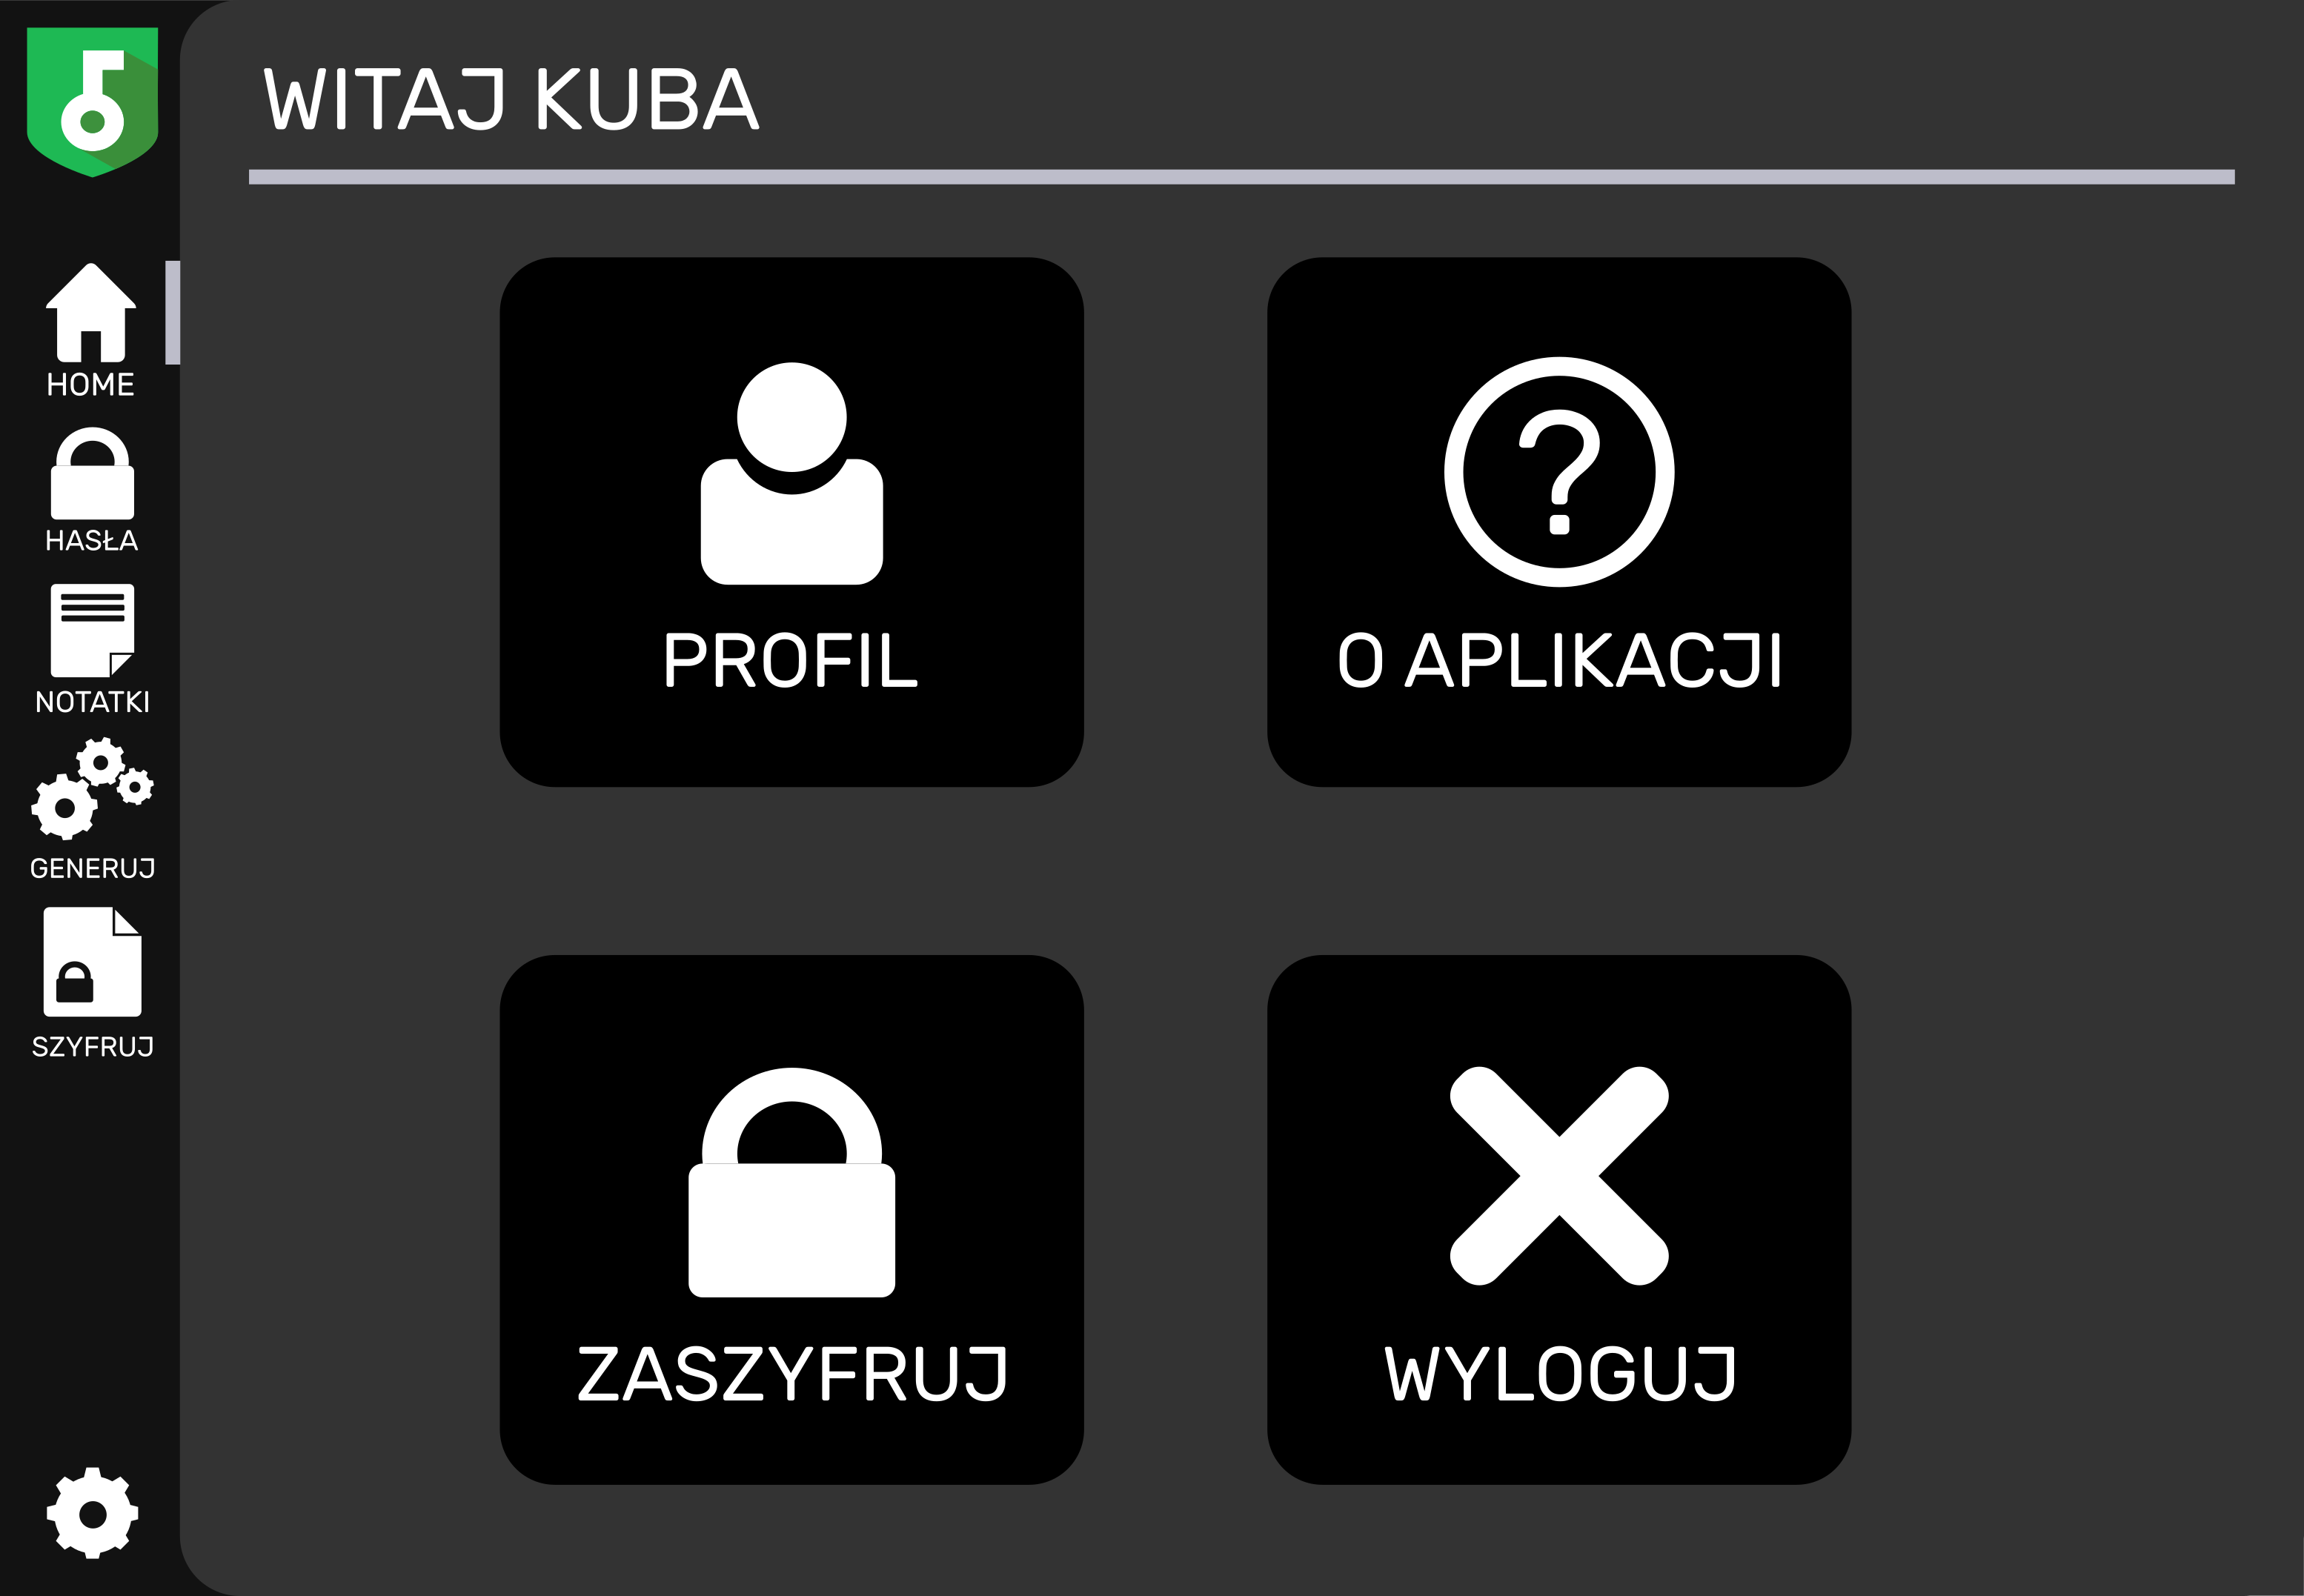
\includegraphics[width=\textwidth]{img/diagrams/ekran_po_zalogowaniu.png}
    \caption{Diagram klas ekranu po zalogowaniu}
    \label{fig:diagramPoL}
\end{figure}
\begin{figure}[H]
    \centering
    \includegraphics[width=\textwidth]{img/diagrams/ekran_haseł.png}
    \caption{Diagram klas ekranu haseł}
    \label{fig:diagramH}
\end{figure}
\begin{figure}[H]
    \centering
    \includegraphics[width=\textwidth]{img/diagrams/ekran_notatek.png}
    \caption{Diagram klas ekranu notatek}
    \label{fig:diagramN}
\end{figure}
\begin{figure}[H]
    \centering
    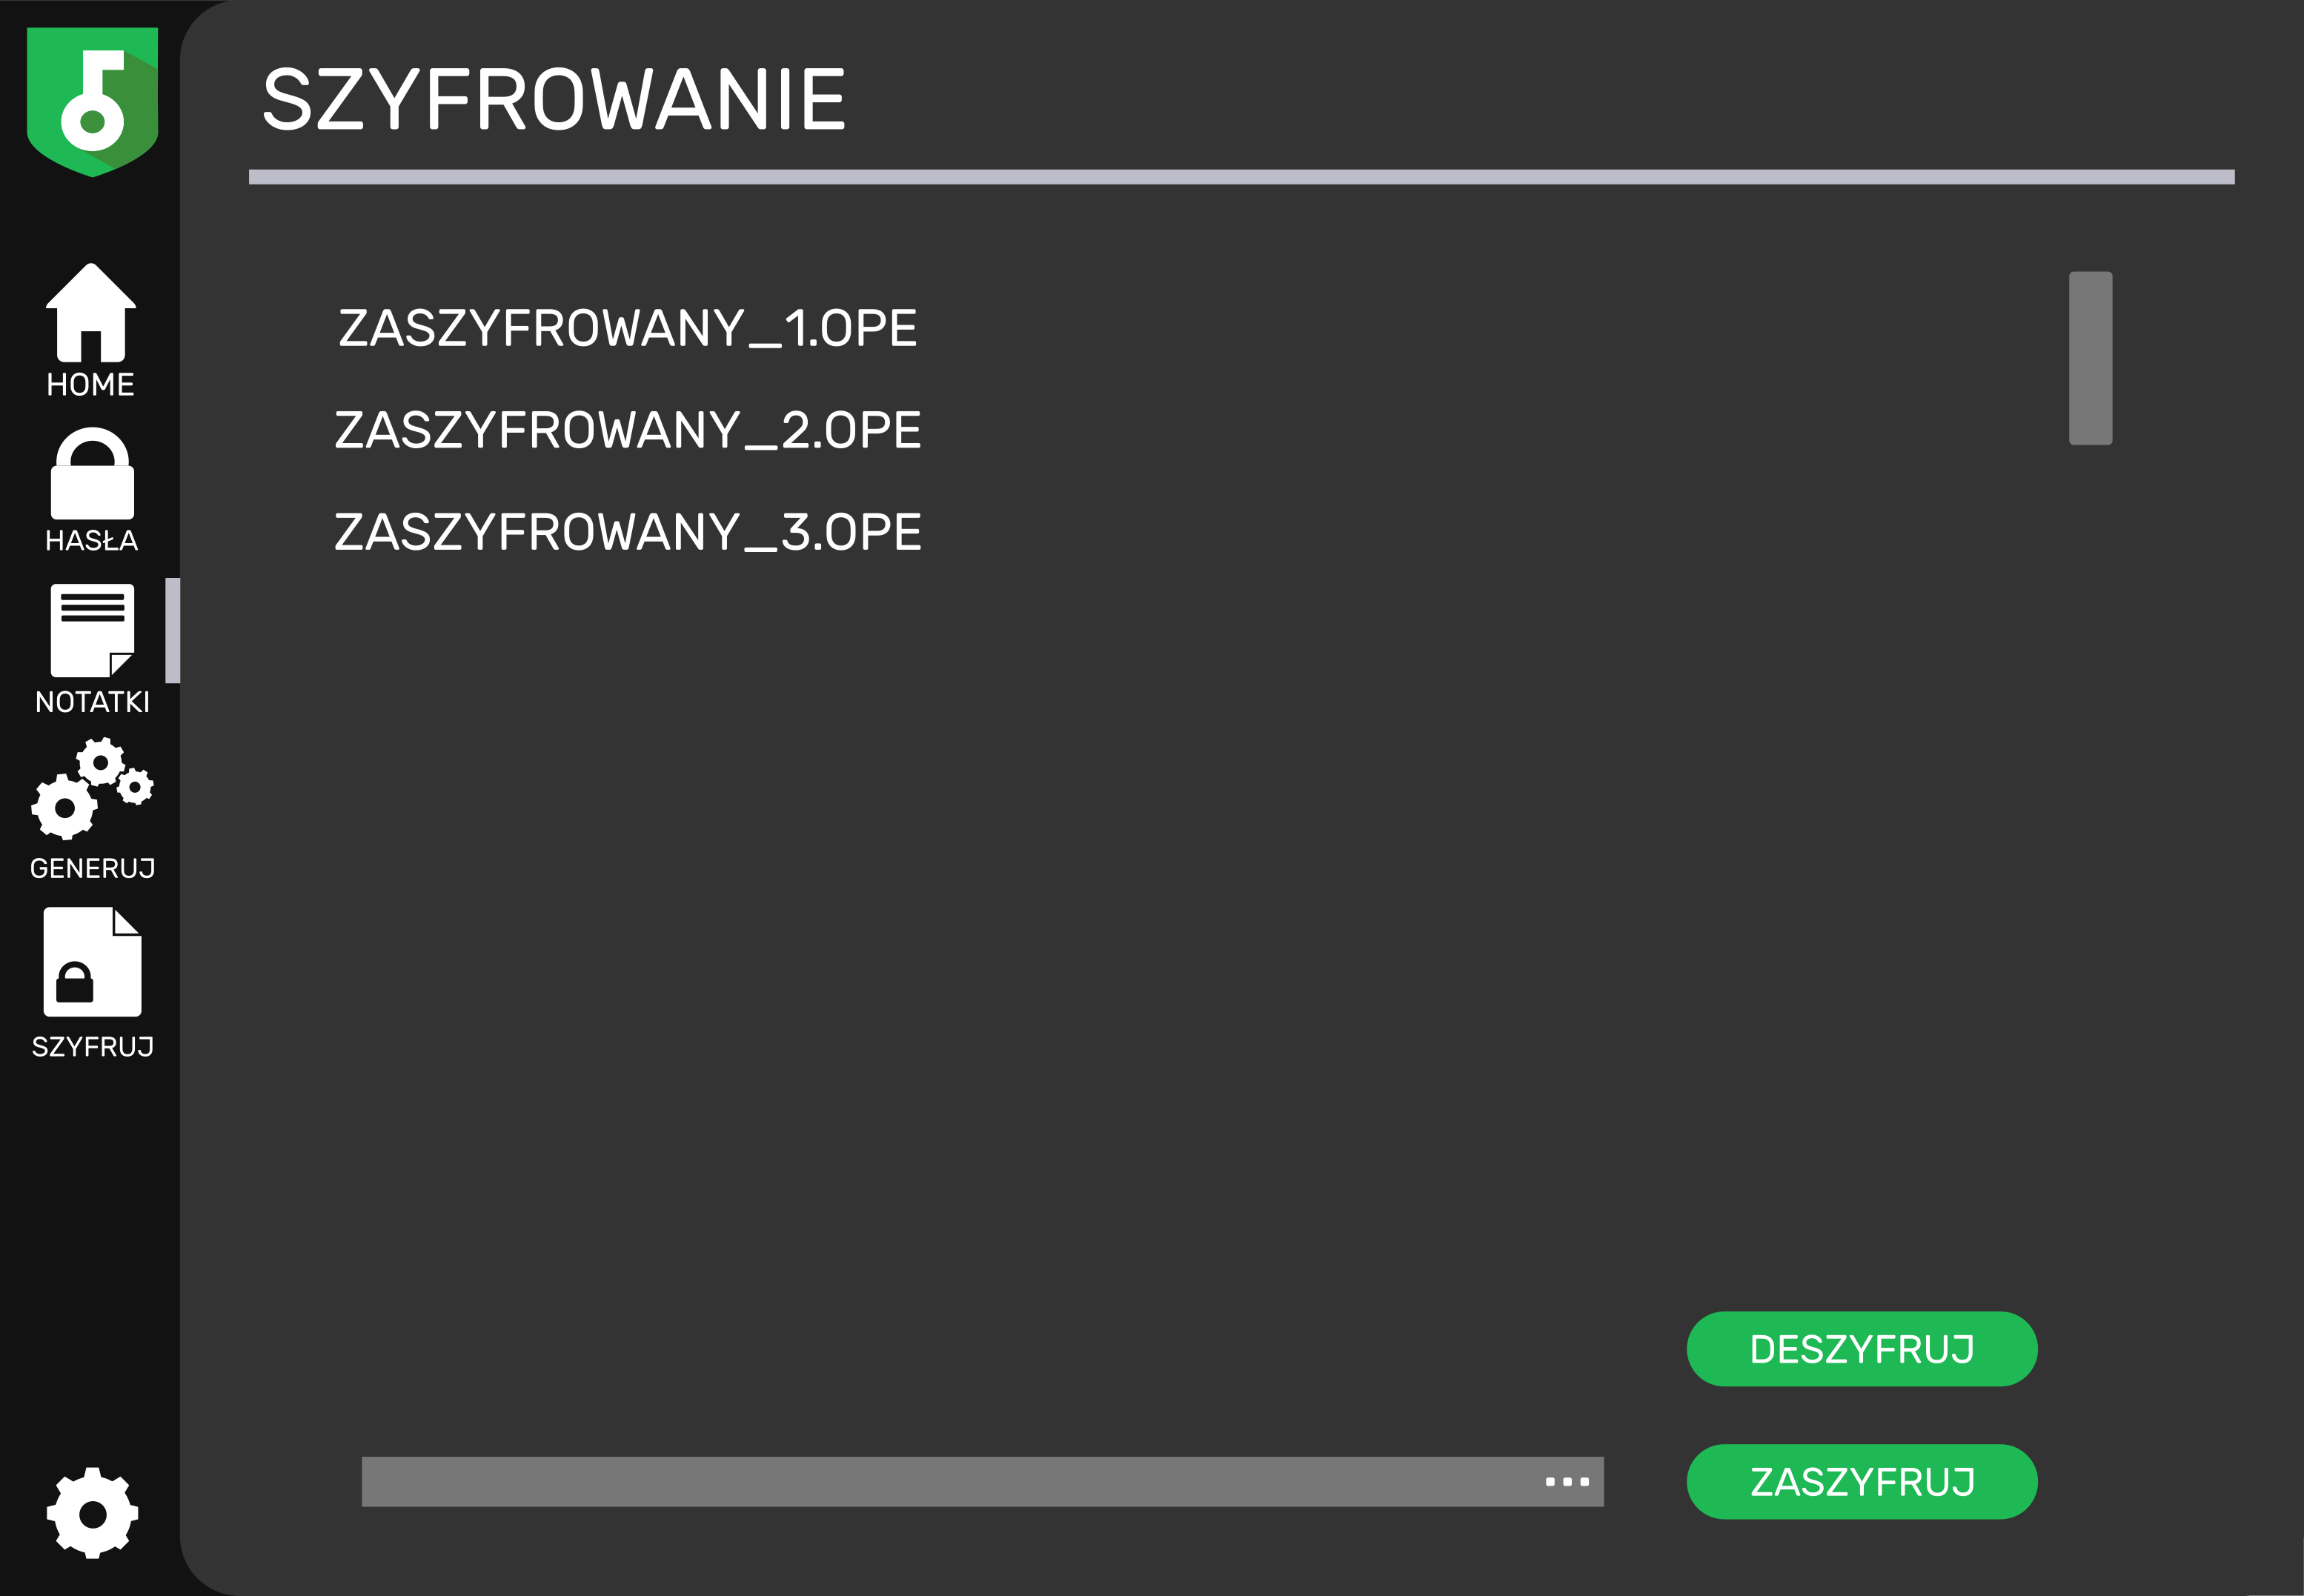
\includegraphics[width=\textwidth]{img/diagrams/ekran_szyfrowania.png}
    \caption{Diagram klas ekranu szyfrowania}
    \label{fig:diagramSz}
\end{figure}
\label{end}

\end{document}